% se puede agregar la opción [english] para 
%  memorias o tesis en inglés (borrando el archivo .aux)
\documentclass[english]{umemoria} 

\depto{Departamento de Física}
\author{Martin Lukas Bataille Gonzalez}
\title{Dynamics of particle-like solutions in non-local systems}

% incluir ambos comandos para una doble titulación
%  o quitar el comando que no aplica
% \memoria{Ingenier[o/a?] Civil en ???}
\tesis{Magíster en Ciencias mención Fisica}
%\tesis{Doctor en ???} % incluir solo este comando para doctorados

% puede haber varios profesores guía seperados por coma;
% pero si es una memoria, solo puede haber un profesor guía
\guia{Marcel Clerc Gavilan} 

% puede haber varios profesores co-guía seperados por coma;
% pero si es una memoria, el profesor co-guía será el primer
% integrante de la comisión
%\coguia{Nombre Completo Co-Guía} % incluir en caso de co-guía de *tesis*

%\cotutela{Nombre Institución} % incluir en caso de cotutela

\comision{Marcel Clerc, Karin Alfaro, Oleh Omel'chenko, Ignacio Bordeu, Mustapha Tlidi}

%\auspicio{Nombre Institución} % incluir en caso de recibir financiamiento

% tiene que ser el año en que se da el examen de título/grado (defensa)
%\anho{2021} % incluir solo para reemplazar el año actual

\usepackage{lipsum}
\usepackage{amsmath}
\usepackage{bm}
\usepackage{svg}
\usepackage{graphicx}
\usepackage{sidecap}
\usepackage{pdfpages}
\setlength{\marginparwidth}{2cm}
\usepackage{todonotes}
\usepackage[sorting=none, citestyle=numeric-comp]{biblatex}
\bibliography{bibliografia}

\begin{document}

\theoremstyle{definition}
\newtheorem{exmp}{Example}[section]
\newcommand{\matr}[1]{\mathbf{#1}}

\frontmatter
\maketitle


\begin{resumen}
    Esta tesis está dedicada al estudio y caracterización de la dinámica de estructuras
    localizadas en sistemas no locales. Más específicamente, este trabajo abarca el estudio de dos
    tipos de estructuras localizadas en sistemas distintos, a saber, solitones disipativos
    en una cavidad de fibra de cristal fotónico, y quimeras espirales en arreglos bidimensionales
    de osciladores de fase acoplados no localmente. En ambos sistemas, se observa la aparición
    de estructuras localizadas móviles mediante distintos mecanismos, los cuales son correspondientemente identificados y discutidos.

    En el Capítulo~\ref{ch:intro}, se presenta una breve introducción a las estructuras localizadas y a los sistemas no locales,
    junto con el alcance y los objetivos de esta tesis. El Capítulo~\ref{ch:preliminary} proporciona los conceptos teóricos esenciales
    necesarios para comprender los capítulos siguientes, mientras que el Capítulo~\ref{ch:continuation} introduce el método de continuación
    numérica empleado en los capítulos posteriores.

    La primera parte de la investigación realizada en esta tesis se compone de los Capítulos~\ref{ch:isolas} y~\ref{ch:filtering},
    y está dedicada al estudio de solitones disipativos en cavidades de fibra de cristal fotónico bajo distintos efectos no locales.
    En particular, el Capítulo~\ref{ch:isolas} está dedicado a la caracterización y análisis de solitones brillantes y oscuros
    móviles sujetos al efecto Raman y considerando dispersión de cuarto orden. Un sistema similar
    es considerado en el Capítulo~\ref{ch:filtering}, con la diferencia de que los dos términos anteriores
    son reemplazados por un filtro espectral, que surge de la adición de una rejilla de fibra al sistema.

    La segunda parte está compuesta por los Capítulos~\ref{ch:spirals} y~\ref{ch:travelingspirals},
    y se centra en quimeras espirales móviles en poblaciones de osciladores de fase acoplados. Comenzando
    con el Capítulo~\ref{ch:spirals}, se revela la existencia de estas estructuras, y se caracteriza su
    dinámica basada en simulaciones numéricas. Posteriormente, el Capítulo~\ref{ch:travelingspirals}
    profundiza el análisis a través del método de continuación numérica y métodos semi-analíticos, proporcionando
    una descripción detallada de la aparición y estabilización de quimeras espirales móviles.

    Finalmente, el Capítulo~\ref{ch:conclu} presenta las principales conclusiones de esta tesis.
\end{resumen}

\begin{abstract}
    This dissertation is devoted to the study and characterization of the dynamics of localized structures
    in non-local systems. More specifically, we focus on two different kind of localized structures
    arising in different systems, 
    namely, dissipative solitons in a photonic crystal fiber cavity, and
    spiral chimeras in two-dimensional arrays of nonlocally coupled phase oscillators. In both 
    systems, we observe the emergence of moving localized structures due to distinct mechanisms,
    which we identify and discuss.

    In Chapter~\ref{ch:intro}, a brief introduction to localized structures and nonlocal systems
    is presented, along with the scope and objectives of this thesis. Chapter~\ref{ch:preliminary}
    provides the essential theoretical concepts needed to understand the following chapters, 
    while Chapter~\ref{ch:continuation}
    introduces the numerical continuation method employed in the subsequent Chapters.
    
    The first part of the research made in this dissertation consists of Chapters~\ref{ch:isolas} and~\ref{ch:filtering},
    and is dedicated to the study of dissipative solitons in photonic crystal fiber cavities under different nonlocal effects.
    In particular, Chapter~\ref{ch:isolas} is dedicated to the characterization and analysis of moving bright and dark
    subject to the Raman effect and considers fourth order dispersion. A similar system 
    is considered in Chapter~\ref{ch:filtering}, with the difference that the two former terms 
    are replaced by a spectral filter, arising from the addition of a fiber grating to the system.
    
    The second part is composed of Chapters~\ref{ch:spirals} and~\ref{ch:travelingspirals}, 
    and focuses on moving spiral chimeras in populations of coupled phase oscillators. Starting
    with Chapter~\ref{ch:spirals}, the existence of these structures is revealed, and their 
    dynamics are characterized based on numerical simulations. Subsequently, Chapter~\ref{ch:travelingspirals}
    deepens the analysis through numerical continuation and semi-analytical methods, providing
    a detailed description of the emergence and stabilization of moving spiral chimeras.
    
    Finally, Chapter~\ref{ch:conclu} presents the main conclusions of this dissertation.
\end{abstract}

\begin{dedicatoria}
tbd. \\
- tbd.
\end{dedicatoria}

\begin{thanks}
    tbd
\end{thanks}



\tableofcontents
% \listoftables % opcional
% \listoffigures % opcional

\mainmatter

\chapter{Introduction}

\label{ch:intro}

Almost a century ago, our understanding of elementary or quantum particles went
through a complete change of paradigm. Indeed, what was originally thought
to be a microscopic speck of matter with a well-defined position, momentum and size
was discovered instead to be a localized field that occupies all space, 
and whose amplitude is related to the probability 
density~\cite{merzbacher1998quantum,messiah2014quantum,gross1962particle}.
As a consequence,
the former quantities of position and momentum were replaced by expectation values.
Conversely, the concept of a particle as a localized field was extended to 
meso- and macroscopical systems, typically described by extended fields.
In fact, Nicolis and Prigogine argued that the energy transfer present in these systems
allows for a rich variety of complex and stable structures to form, including localized 
structures~\cite{prigogine1977self, pismen2006patterns}.
These localized states or particle-like solutions are thus supported by a robust balance between 
gains and losses and have been observed in a variety of systems due to their 
universality~\cite{umbanhowar1996localized,aranson2006patterns,minardi2010three,verschueren2013spatiotemporal,yi2018imaging}. 

Traditionally, the mathematical description of localized structures has been carried out using
reaction diffusion models or their generalizations with higher order 
derivatives~\cite{tlidi1994localized,coullet2000stable,knobloch2015spatial}.
As the name suggests, the spatial coupling occurs through diffusive (or hyperdiffusive) terms and, 
therefore, is solely local. Nevertheless, various optical~\cite{gelens2007impact}, 
neural~\cite{coombes2005waves} and even vegetation~\cite{lefever1997origin} systems present a more 
complex and far-reaching coupling, usually called nonlocal coupling. In these cases,
it has been found that the nonlocal term gives rise to richer dynamics and is often responsible for the
stabilization of particle-like solutions~\cite{fernandez2013strong, clerc2020time}. Mathematically, the nonlocal term is usually modeled as an
integral operator, which strongly limits the analytical and numerical tools available to study these systems.
Consequently, the dynamics of localized structures in nonlocal systems are still not well understood.

The aim of this dissertation is to provide an in-depth study and characterization of
the dynamics of localized structures in non-local systems. In particular, we will focus 
on two different systems: dissipative solitons in a photonic
crystal fiber cavity, and spiral chimeras in two-dimensional networks of heterogeneous phase oscillators. 
In both cases, we observe the emergence of uniformly moving localized structures due to different mechanisms,
which we will identify and analyze.

\section{Contents}

This dissertation is a compilation of four articles that have been published or submitted to peer-reviewed journals.
For each article, there is an associated chapter containing a brief introduction to the subject, 
along with a short discussion at the end. 

The first three chapters of this dissertation are dedicated
to the theoretical and numerical background necessary for the subsequent chapters. More specifically,
Chapter~\ref{ch:intro} corresponds to the present introduction, and provides an overview of the context and 
scope of the dissertation. Chapter~\ref{ch:preliminary} introduces the main concepts and theory needed 
to approach the current study. In Chapter~\ref{ch:continuation}, an introduction to numerical continuation,
the main numerical method used in the following articles, is presented. 

The following four chapters contain the core of the dissertation, which is divided into two main parts. The first
part contains Chapters~\ref{ch:isolas} and~\ref{ch:filtering}, and focuses on dissipative solitons in photonic crystal 
fiber cavities, under different asymmetric nonlocal effects. Starting with Chapter~\ref{ch:isolas},
the formation of isolas of solitons due to the Raman effect is studied. In Chapter~\ref{ch:filtering}, a similar 
system is considered under a different nonlocal coupling, arising from the addition of a spectral filter.

On the other hand, the second part of the dissertation is devoted to the study of moving spiral wave chimeras
in a two-dimensional array of nonlocally coupled phase oscillators. In particular, Chapter~\ref{ch:spirals}
reveals the existence of these structures and characterizes their dynamics based on direct numerical simulations.
Chapter~\ref{ch:travelingspirals} extends the analysis through numerical continuation and semi-analytical methods,
and provides a detailed description of the bifurcations that lead to the creation, stabilization and disappearence of
moving spiral chimeras. Finally, Chapter~\ref{ch:conclu} presents the main conclusions of this thesis.


\section{Objectives}
The main objective of this dissertation is to study and characterize the creation, stabilization and disappearence
of propogative localized structures in nonlocal systems. To achieve this, the following specific objectives were proposed.
\begin{itemize}
  \item Identify and understand the different physical mechanisms responsible for the propagation of
  localized structures.
  \item Classify the different types of dynamics through an extensive exploration of the parameter space.
  \item Develop and implement a numerical method for the continuation of complex traveling solutions in
  one- and two-dimensional nonlocal systems.
  \item Identify and characterize the bifurcations that lead to the creation, stabilization and disappearence 
  of localized structures through the use of numerical continuation techniques.
\end{itemize}

\section{Common abbreviations}

\begin{itemize}
  \item {\bf LS}: Localized structures
  \item {\bf DS}: Dissipative soliton
  \item {\bf SHE}: Swift-Hohenberg Equation
  \item {\bf LLE}: Lugiato-Lefever Equation
  \item {\bf NLS}: Nonlinear Schrödinger Equation
  \item {\bf KdV}: Korteweg-de Vries Equation
  \item {\bf HSS}: Homogeneous Steady State
  \item {\bf SRS}: Stimulated Raman Scattering
\end{itemize}

\section{Contribution statement}

\subsection{Isolas of localized structures and Raman–Kerr frequency combs in micro-structured resonators (Chaos, Solitons \& Fractals 174, 113808)}
Marcel G. Clerc and Mustapha Tlidi conceptualized the study and designed the research. 
{\bf Martin Bataille-Gonzalez} implemented and performed numerical simulations and continuation. 
Marcel G. Clerc and Mustapha Tlidi wrote the manuscript. {\bf Martin Bataille-Gonazalez} 
contributed to editing and revising the manuscript.


\subsection{Dissipative Soliton Combs with Spectral Filtering. (submitted to Physical Review A)}
Marcel G. Clerc and Mustapha Tlidi conceptualized the study and designed the research. {\bf Martin Bataille-Gonzalez},
Bilal Kostet and Youri Soupart performed research (numerical integration, implementation of numerical continuation, and analysis of numerical data).
Bilal Kostet and Mustapha Tlidi developped the analytical framework.
Bilal Kostet, Youri Soupart, Mustapha Tlidi and Marcel Clerc wrote the manuscript. 
{\bf Martin Bataille-Gonazalez} contributed to editing and revising the manuscript.

\subsection{Moving spiral wave chimeras (Physical Review E, 104(2), L022203)}
Oleh Omel'chenko conceptualized the study and designed the research. {\bf Martin Bataille-Gonzalez} performed research (numerical integration, and analysis of numerical data).
Marcel G. Clerc supervised the research and provided critical feedback. Oleh Omel'chenko and Marcel G. Clerc wrote the manuscript. 
{\bf Martin Bataille-Gonazalez} contributed to editing and revising the manuscript.

\subsection{Traveling spiral wave chimeras in coupled
oscillator systems: emergence, dynamics, and
transitions (New Journal of Physics 25, 103023)}
Oleh Omel'chenko conceptualized the study and designed the research. 
{\bf Martin Bataille-Gonzalez} and Oleh Omel'chenko implemented and performed numerical simulations and continuation.
Marcel G. Clerc and Edgar Knobloch supervised the research and provided critical feedback. Oleh Omel'chenko and Edgar Knobloch wrote the manuscript. 
{\bf Martin Bataille-Gonazalez} and Marcel G. Clerc contributed to editing and revising the manuscript.
\chapter{Preliminary concepts}

\section{Dynamical Systems}

[introducir bien el tema]. 

The general form for a dynamical system will be the following.

\begin{equation}
    \dfrac{d\bm{u}}{dt} = \bm{f}(\bm{u}, \eta), \qquad \bm{f} : \mathbb{R}^N \times \mathbb{R}^{n_\eta} \to \mathbb{R}^N
    \label{eq:def_ds}
\end{equation}

Here, $\bm{u}$ represents the state vector of the system, it might correspond to the
concentrations of different chemicals, the population of certain species or the amplitude
of an electric field. The temporal evolution of the state of the system is thus determined by 
the vector function $\bm{f}$. This function may in turn depend on one or several control
parameters $\eta$ relevant to the modeled experiment such as
[Agregar parametros]

In this thesis, we will consider different dynamical systems represented by Eq.~(\ref{eq:def_ds}) where the function
$\bm{f}$ will be {\em nonlinear}. Although one might argue that, at a fundamental level, the physical laws
that describe the evolution of a system (Schrödinger equation for example) are linear, when one looks at meso- or macroscopical
systems, nonlinear terms naturally arise due to the coarse-graining of the microscopical degrees of freedom [ref Karadr].


In the case of a nonlinear dynamical system, it becomes extremely difficult, and often impossible, to find
general explicit solutions of Eq.~(\ref{eq:def_ds}). But it turns out that in most cases an in depth
description of the model can be provided by studying only the steady states ($\bm{f}(\bm{u}, \eta) = 0$) and their qualitative changes as parameters 
are varied. In other words, the problem can be reduced as to find the {\em equilibria} and {\em bifurcations} of the system.
In the following section, we shall describe the simplest bifurcations a system can experience.

\section{Bifurcations}

Qualitative changes of equilibria as parameters are varied.

% Ideas:
% \begin{enumerate}
%     \item saddle-node for genes pp 249
%     \item magnetism Landau Pitchfork
%     \item Hopf, van der pol, bici
% \end{enumerate}

\subsection{Saddle-Node bifurcation}

{\em Saddle-node} or {\em fold} bifurcations provide the simplest mechanism 
for which a pair of stable and unstable equilibria can be created (or destroyed) 
as the control parameter is changed. Although they arise in a huge variety of systems 
[insert ref], close to the bifurcation point the dynamics can always be reduced to
the following minimal or {\em normal form}.

\begin{equation}
    \dfrac{du}{dt} = \eta - u^2
    \label{eq:pre_bif_sn}
\end{equation}

Following the notation of Eq.~(\ref{eq:def_ds}), u represents the state variable
and $\eta$ the control parameter. For $\eta > 0$, the system presents two equilibria $u_{\pm} = \pm\sqrt{\eta}$, where $u_+$ is
stable and $u_-$ unstable. An interesting case occurs when $\eta = 0$, at which point $u = 0$ is
half-stable (stable for positive perturbations and unstable for negative perturbations). Lastly,
for $\eta < 0$ there are no equilibria. Figure~(\ref{fig:pre_bifs_sn}) provides a visual representation
of the previous analysis.

In short, as the bifurcation parameter $\eta$ is decreased (increased)
starting from positive (negative) values, the two equilibria attract (repel) each other and suddenly annihilate (appear).

\begin{figure}[h]
    \centering
    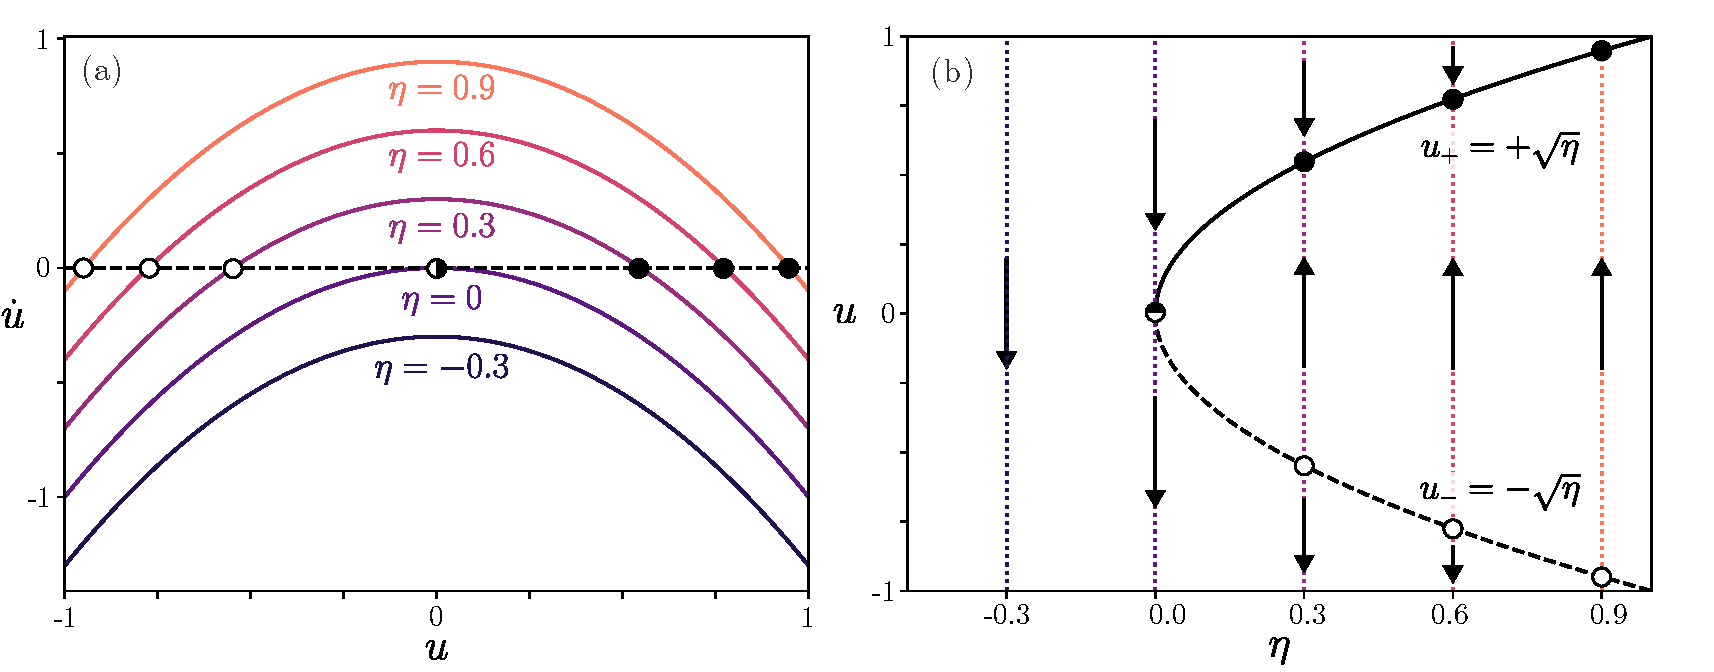
\includegraphics[width=\textwidth]{imagenes/framework/bif_sn_f.pdf}
    \caption{Prototipical scenario for a saddle-node bifurcation. (a) Phase space
    showing both stable and unstable fixed points for different values of $\eta$. 
    Black (white) circles represent
    stable (unstable) fixed points. (b) Bifurcation diagram showing
    the creation of a stable-unstable pair of fixed points. Solid (dashed) line represents
    stable (unstable) branch.}
    \label{fig:pre_bifs_sn}
\end{figure}

\begin{exmp}
    For centuries, the mystery of synchronization between fireflies has
    captivated many people. Although many open questions remain on this topic [ref],
    we will aim to shed {\em light} on this topic only with the knowledge of saddle-node bifurcations
    and a simple model proposed by Ermentrout and ...[ref]. 
    
    Consider the problem
    of a firefly flashing under the presence of a periodically flashing light.
    We will model the flashing of the firefly with an angular variable $\theta$
    such that $\theta = 0$ represents the firefly's flash. The firefly has its 
    own inherent frequency $\omega$, i.e. in the absence of stimuli 
    $\dot{\theta} = \omega$. On the other hand, the periodic stimulus will be
    represented by a phase $\phi$ that satisfies $\dot{\phi} = \Omega$, where 
    $\Omega$ is of course the stimuli period. In order to synchronize with the
    stimuli, the firefly will either want to speed up if it is lagging behind
    or slow down if it is going too fast. The simplest non-linear model that
    fulfills these assumptions is the following,
    \begin{align*}
        \dot{\phi} &= \Omega \\
        \dot{\theta} &= \omega + A \sin(\phi -  \theta)
    \end{align*}

    Subtracting both equations and defining $\varphi = \dot{\phi} - \dot{\theta}$
    yields 

    \begin{equation*}
        \dot{\varphi} = \Omega - \omega - A \sin \varphi
    \end{equation*}

    which can be adimensionalized by rescaling $t \to At$ and introducing
    the non dimensional parameter $\mu = (\Omega - \omega)/A$,

    \begin{equation}
        \dot{\varphi} = \mu - \sin \varphi
        \label{eq:pre_bif_sn_exmp}
    \end{equation}

    For $\mu = 0$ where the forcing and intrinsic frequencies are the same, there
    is a stable fixed point at $\varphi = 0$ and an unstable fixed point at $\varphi = \pi$.
    As $\mu$ increases, both equilibria approach each other until they collide for $\mu=\mu_c=1$
    at $\varphi = \pi/2$
    and then disappear for $\mu > 1$. We can clearly recognize that the pair of fixed
    points appear (or disappear) through a saddle-node bifurcation.
    
    Moreover, close to the bifurcation point where $\mu_c = 1$ and $\varphi_c = \pi/2$,
    we can do a Taylor expansion: $\mu = 1 + \eta$ and $\varphi = \pi/2 + u$ 
    where $\eta, u \ll 1$. Using the identity $\sin \varphi = \sin (\pi/2 + u) = \cos u$
    and inserting the previous ansatz into Eq.~(\ref{eq:pre_bif_sn_exmp}) yields
    the following
    \begin{align*}
        \dot{\varphi} = \dot{u} &= 1 + \eta - \cos u \\ 
        &\approx 1 + \eta - (1 - \dfrac12 u^2) \\
        &= \eta - \dfrac12 u^2
    \end{align*}

    Which after adequate rescaling corresponds exactly with the saddle-node
    normal form.
    

\end{exmp}

\subsection{Pitchfork bifurcation}

A {\em pitchfork} bifurcation constitutes the simplest symmetry-breaking bifurcation.
Its normal form is given by

\begin{equation}
    \dfrac{du}{dt} = \varepsilon u - u ^ 3
\end{equation}

Note that the above formula corresponds to a {\em supercritical} bifurcation, the emerging branches from the
bifurcation point are stable. On the contrary, in the {\em subcritical} case, the cubic
term should be positive and a negative quintic term should be added to ensure the solution is bounded.
\subsection{Hopf bifurcation}

[insert example]

\section{Localized Structures}
\label{sec:fra_LS}

\subsection{Solitons}
\subsection{The Lugiato-Lefever equation}

\section{Phase oscillators and Chimera states}
\subsection{Phase oscillators}

\subsection{Kuramoto model}

\subsection{Spiral wave chimeras}
\chapter{Numerical Continuation}

As stated in the previous section, we will be interested in following the solution
branches as it experiences several bifurcations. Since an analytical treatment is not
usually available for the problems studied in this work, we must resort to numerical methods.
Namely, we will implement and develop a numerical continuation algorithm. These type of methods
aim to solve a nonlinear equation or, more generally, a system of nonlinear equations in order to find the desired steady states of a dynamical system 
as parameters are changed. This task corresponds to finding the roots (zeros) of a vector function $\bm{F}$, as in Eq.~(\ref{eq:pre_nc_zeros}). 
We will assume we previously know a solution $\bm{u}_0$ for a certain parameter $\eta_0$, obtained
for example through numerical simulation.

\begin{equation}
    0 = \bm{F}(\bm{u}, \eta)
    \label{eq:pre_nc_zeros}
\end{equation}

Although there are several methods for finding the roots of a vector function,
in this thesis we will only use Newton's method because of its fast (quadratic) convergence
and simplicity. Recall that Newton's method is an iterative method that given an initial
guess $\bm{u_0}$ will perform successive iterations until a certain accuracy or tolerance
is reached. Each iteration is computed using Eqs~(\ref{eq:pre_nc_newt1}-\ref{eq:pre_nc_newt2}),
where $\matr{J}(\bm{u}_i, \eta)$ is the Jacobian of $\bm{F}$. Moreover, since we have access
to the Jacobian in Newton's method, we can track the stability of the solution and detect bifurcation
points by tracking changes in the sign of the determinant of the Jacobian.

\begin{align}
    \matr{J}(\bm{u}_i, \eta) \Delta \bm{u}_{i+1} &= - \bm{F}(\bm{u}_i, \eta) 
    \label{eq:pre_nc_newt1}
    \\
    \bm{u}_{i+1} &= \bm{u}_i + \Delta \bm{u}_{i+1}
    \label{eq:pre_nc_newt2}
\end{align}

\section{Natural parameter continuation}

The simplest way to perform numerical continuation is to fix the value of the parameter, in this case $\eta$, and solve
the equation (or system of equations) by means of Newton's method. Then, one can increase the 
parameter by a small step $\eta = \eta_0 + \Delta \eta$ and find the new solution using 
the previous solution $\bm{u_0}$ as initial guess for Newton's method. Finally, we repeat the process
until the whole solution branch has been computed. This method is usually called {\em Natural Parameter Continuation}
\cite{doedel2007lecture}.

\begin{exmp}
    In order to illustrate the method lets consider a simple
    example: finding the homogeneous solutions to the Swift-Hohenberg equation. More specifically,
    we will look for both the stable and unstable equilibria of Eq.~(\ref{eq:pre_nc_she}).    
    \begin{equation}
        \dot{u} = \eta + \varepsilon u - u^3
        \label{eq:pre_nc_she}
    \end{equation}

    This is the same
    as to find the roots of a cubic polynomial: $F(u, \eta) = \eta + \varepsilon u - u^3 = 0$. The derivative
    can be determined easily: $J(u, \eta) = \varepsilon - 3u^2$. 
    %Moreover, when $\eta=0$, $F$ admits three distinct real solutions when
    % $\varepsilon$ is positive and one real and two complex conjugate roots when $\varepsilon$ is negative. 

    We will look at the case where $\varepsilon = 0.1$, for which the system is bistable. Indeed, if we start the algorithm
    at $\eta=-0.02$ taking as initial guess $u_0 = -0.4$ and perform a forward sweep (slowly increasing $\eta$), and then
    repeat the process backwards we obtain Fig.~(\ref{fig:pre_nc_she}).

    \begin{figure}[h]
        \centering
        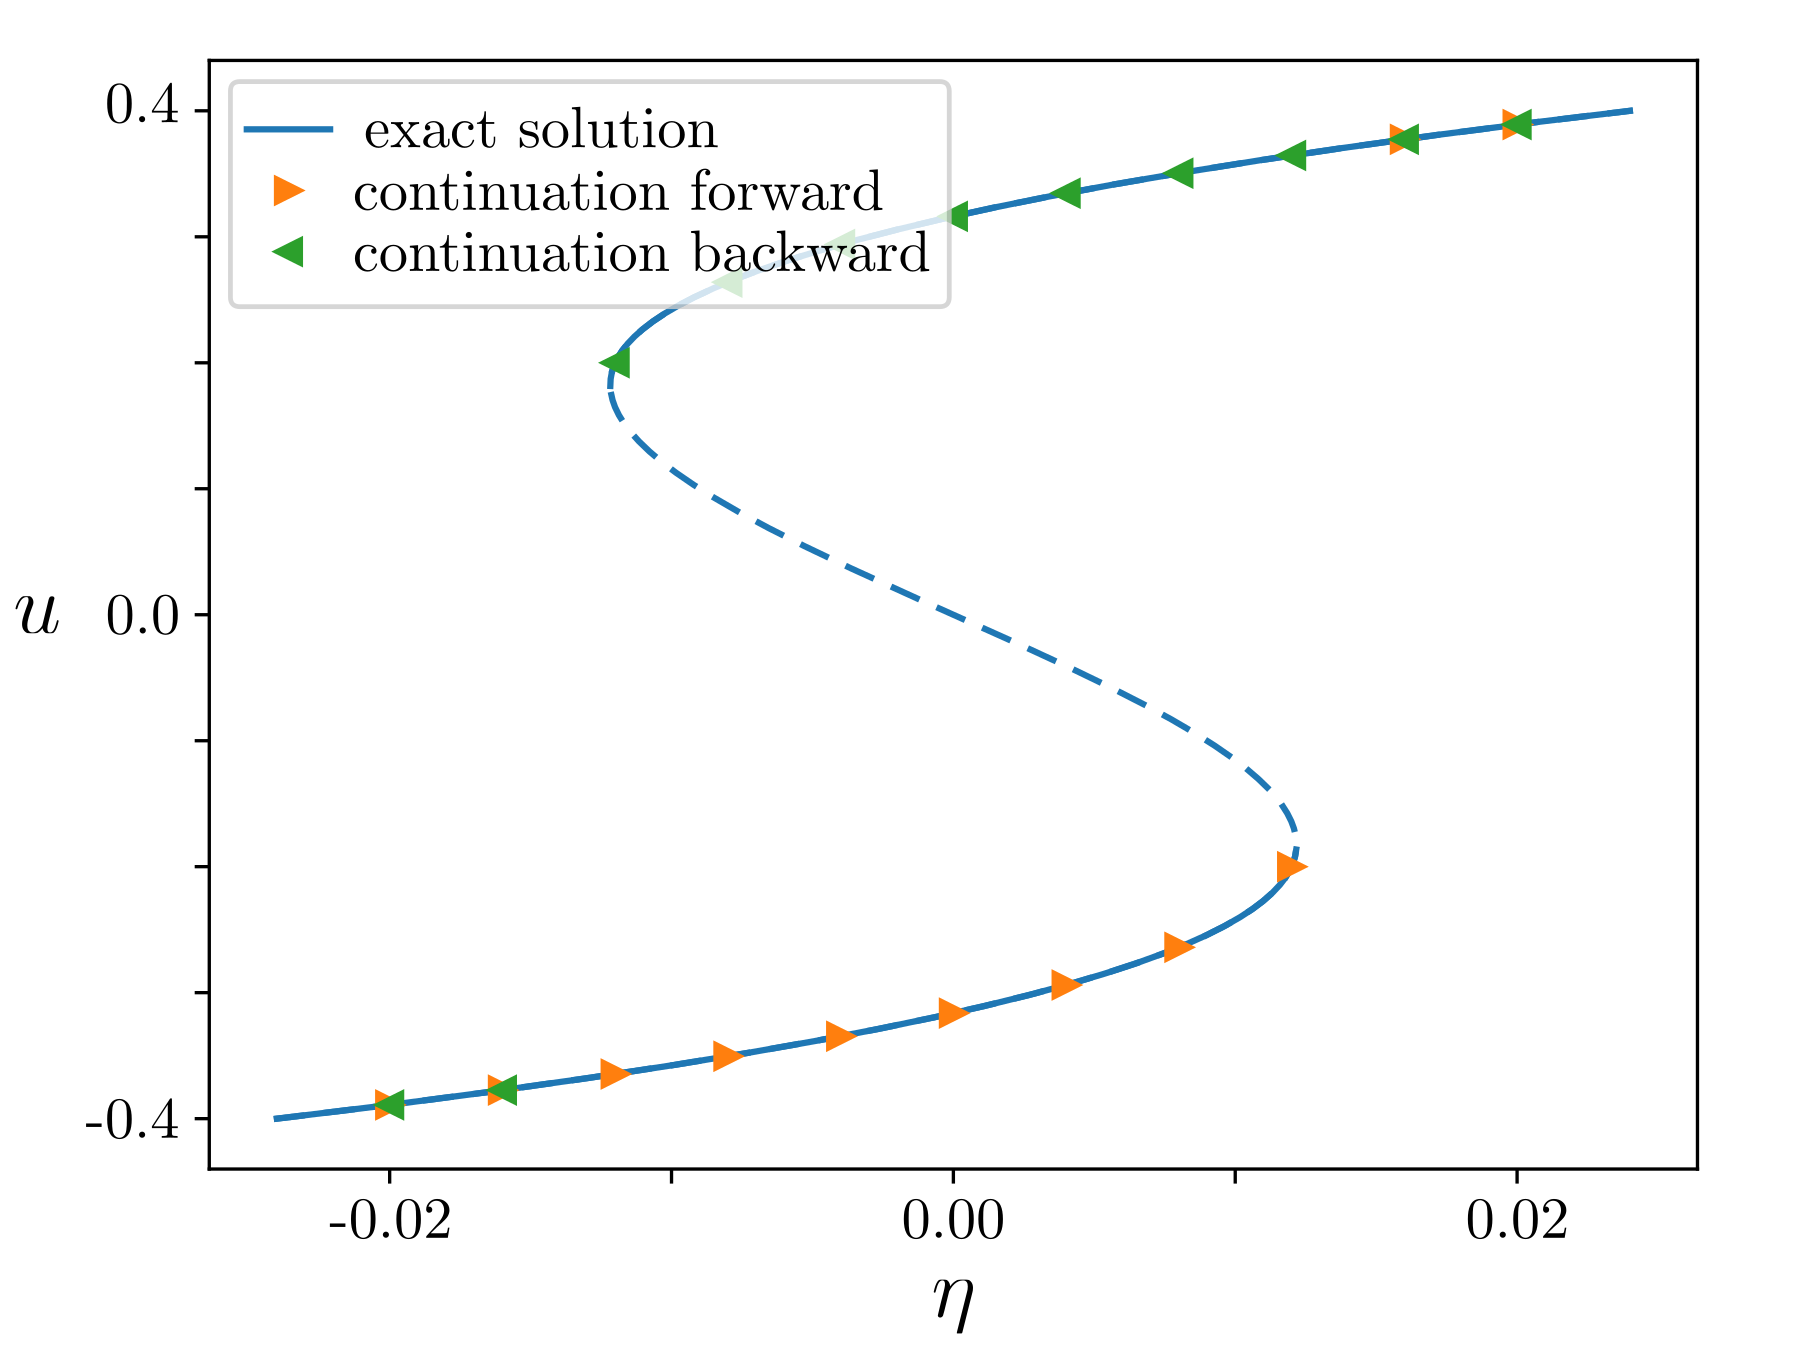
\includegraphics[width=0.7\textwidth]{scripts/figures/natural_continuation_she.png}
        \caption[short]{Solution of Eq.~(\ref{eq:pre_nc_she}) as a function of the parameter $\eta$ obtained
        through natural continuation (orange and green triangles) compared to the exact solution (blue curve).}
        \label{fig:pre_nc_she}
        %\includesvg[width=0.5\textwidth]{scripts/figures/natural_continuation_she.svg}
    \end{figure}
\end{exmp}

Note that the natural continuation succeeded at finding the lower and upper branch of the solution
in this example.
However, it could not follow the branch past the fold (or saddle-node) bifurcation. The
only way to access the middle branch using this algorithm would be to use an adequate initial guess close
to the middle branch. 
Although in this case, it is not difficult to find one, for a higher-dimensional system where the
bifurcation scenario is more complicated, this quickly becomes impractical. To overcome this limitation,
one can implement a more robust continuation scheme: the {\em pseudo-arclength continuation}.

\section{Pseudo-arclength continuation}


As shown in the previous example, $\eta$ is not necessarily the good parameter to describe the curve, as it
does not allow us to follow the branch through a fold point. A different approach can be taken where we
parametrize the solution branch by a different parameter: $s$, which is somewhat similar
to the arc-length. Therefore, our goal is to obtain a set of points 
$\bm{y}(s) = (\bm{u}(s), \eta(s))$.
Then the {\em pseudo-arclength} algorithm \cite{keller1977numerical} consists essentially of two steps that ensure that the branch is followed through folds.
\begin{enumerate}
    \item {\em Predictor step.} Extrapolate a distance $\Delta s$ along the tangent $\bm{\tau}_0$ from a previously known point $(\bm{u}_0, \eta_0)$ in the $(\bm{u},\eta)$ space, to
    obtain the predicted point (the point used as initial guess). 
    $$\bm{y} = \bm{y}_0 + \bm{\tau}_0 \Delta s$$
    \item {\em Corrector step.} Force the solution to stay in the plane perpendicular to the tangent. 
    Or, equivalently, that the solution projected onto the tangent has length $\Delta s$. 
    $$(\bm{y} - \bm{y_0}) \cdot \bm{\tau}_0 = \Delta s$$
\end{enumerate}

We have introduced in these steps a new object: the tangent $\bm{\tau}$ of the solution curve $\bm{y}(s)$,
which is defined as,
\begin{equation}
    \bm{\tau} = \frac{d}{ds}\bm{y} = \left(\frac{d\bm{u}}{ds}, \frac{d\eta}{ds}\right)
\end{equation}

An additional step must therefore be carried out in order to implement this method: computing 
the tangent vector. To do this, it is convenient to revisit Eq.~(\ref{eq:pre_nc_zeros}) and write out
the dependence on the new parameter $s$ explicitly.
\begin{equation}
    0 = \bm{F}(\bm{u}(s), \eta (s))
\end{equation}

We can take the derivative with respect to $s$ on both sides of the
above equation, and obtain the following,
\begin{equation}
    0 = \matr{J}(\bm{u}(s), \eta (s)) \frac{d \bm{u}}{ds} 
            + \bm{F_\eta}(\bm{u}(s), \eta (s)) \frac{d\eta}{ds}
   %  \matr{J}(\bm{x}(s), \eta (s))  \frac{d \bm{x}}{ds} &= -  \bm{F_\eta}(\bm{x}(s), \eta (s)) \frac{d\eta}{ds}
    \label{eq:pre_nc_tangent}
\end{equation}

Additionally, in order to uniquely define the tangent vector, we must
impose a restriction on its length, the most reasonable choice being
to normalize it. Therefore, another equation must be added,

\begin{equation}
    \left|\left|\dfrac{d\bm{u}}{ds}\right|\right|^2 + \left(\dfrac{d\eta}{ds}\right)^2 = 1
    \label{eq:pre_nc_tangent_normalization}
\end{equation}

Then, we can fix $\frac{d \eta}{ds} = 1$ and solve Eq.~(\ref{eq:pre_nc_tangent}) for $\frac{d}{ds}\bm{u}$. Since
it constitutes a system of linear equations, it can be solved using a standard linear solver. Finally, 
the tangent vector must be normalized in order to satisfy Eq.~(\ref{eq:pre_nc_tangent_normalization})
and its sign chosen such that it has the same orientation as the previously
known tangent $\bm{\tau}_0$ i.e. such that $\bm{\tau} \cdot \bm{\tau}_0 > 0$. In the very first step
of the continuation method we do not know a previous tangent, in that case we can choose the
orientation of $\bm{\tau}$ such that its last element (corresponding to  $\frac{d \eta}{ds}$) is
positive if we want to compute the solution branch for increasing values of the parameter $\eta$ or negative
for decreasing values of the parameter.

It is convenient to define an extended vector function $\tilde{ \bm{F} }$ that incorporates $\bm{F}$
and the corrector step in the following manner,
\begin{equation}
    \tilde{\bm{F}}(\bm{y}) = 
    \begin{pmatrix}
        \bm{F}(\bm{y}) \\ 
        (\bm{y} - \bm{y}_0) \cdot \bm{\tau}_0 - \Delta s
    \end{pmatrix}.
    \label{eq:pre_nc_palc_system}
\end{equation} 

And its corresponding Jacobian $\tilde{\matr{J}}$ reads
\begin{equation}
    \tilde{\matr{J}} = 
    \begin{pmatrix}
        \matr{J} & \bm{F}_\eta \\
        \dfrac{d\bm{u}}{ds} & \dfrac{d\eta}{ds} \\
    \end{pmatrix}.
\end{equation}

Notice that the last row of the extended Jacobian $\tilde{\matr{J}}$ corresponds
exactly to the tangent vector $\bm{\tau}$. 

We can summarize the pseudo-arclength continuation algorithm in the following steps.

\begin{enumerate}
    \item Compute a first point in the solution branch $\bm{y}_0 = (\bm{u}_0, \eta_0)$,
    typically through direct numerical simulations. Additionally, one could run
    Newton's method once while keeping the parameter fixed at $\eta = \eta_0$ to obtain
    a more accurate approximation for $\bm{u}_0$.

    \item Solve Eq.~(\ref{eq:pre_nc_tangent}) and find the tangent at that point $\bm{\tau}_0$.
    Choose the orientation of $\bm{\tau}_0$ such that it points in the desired direction on the
    $\eta$-axis.

    \item Using $\bm{y}_0 + \bm{\tau}_0 \Delta s$ as initial guess in Newton's method, solve
    Eq.~(\ref{eq:pre_nc_palc_system}) to find the next point in the solution branch $\bm{y}_{i+1}$.

    \item Again, solve Eq.~(\ref{eq:pre_nc_tangent}) and find the tangent at that point $\bm{\tau}_{i+1}$.
    Choose the orientation such that it matches the previous tangent, $\bm{\tau}_{i+1} \cdot \bm{\tau}_i > 0$.

    \item Repeat steps 3-4 until the whole solution branch has been computed. One could also
    track changes in the sign of the determinant of $\matr{J}$ in order to estimate the location
    of bifurcation points.
\end{enumerate}

% \begin{defn}[ver \cite{KAR00}] Definición definitiva $$\frac{d}{dx}\int_a^xf(y)dy=f(x).$$\end{defn}

\begin{exmp}
    Let's revisit the previous example and implement the pseudo-arclength continuation
    to the same problem. The extended function $\tilde{\bm{F}}(u, {\eta})$ can be written
    in the following form,
    \begin{equation}
        \tilde{\bm{F}}(u, \eta) = 
            \begin{pmatrix}
                \eta + \varepsilon u - u^3 \\
                \left(u - u_0\right) \dfrac{du}{ds} + (\eta - \eta_0) \dfrac{d\eta}{ds} - \Delta s
            \end{pmatrix}.
            \label{eq:pre_nc_palc_she}
    \end{equation}
    Therefore, the extended Jacobian $\tilde{\matr{J}}$ reads,
    \begin{equation*}
        \tilde{\matr{J}} = \begin{pmatrix}
                \varepsilon - 3u^2 & 1 \\
                \dfrac{du}{ds} & \dfrac{d\eta}{ds}
            \end{pmatrix}.
    \end{equation*}

    The tangent vector $\bm{\tau} = (\tau_u, \tau_{\eta})$ can be computed by solving Eq.~(\ref{eq:pre_nc_tangent}).
    We start by fixing $\frac{d}{ds}\eta = 1$, then $\frac{d}{ds}u$ can be obtained directly,
    \begin{equation*}
        \dfrac{du}{ds} = -\dfrac{F_{\eta}}{J} = -\dfrac{1}{\varepsilon - 3u^2}.
    \end{equation*}
    Finally, we normalize $\bm{\tau}$ to obtain the tangent vector.

    \begin{figure}[h]
        \centering
        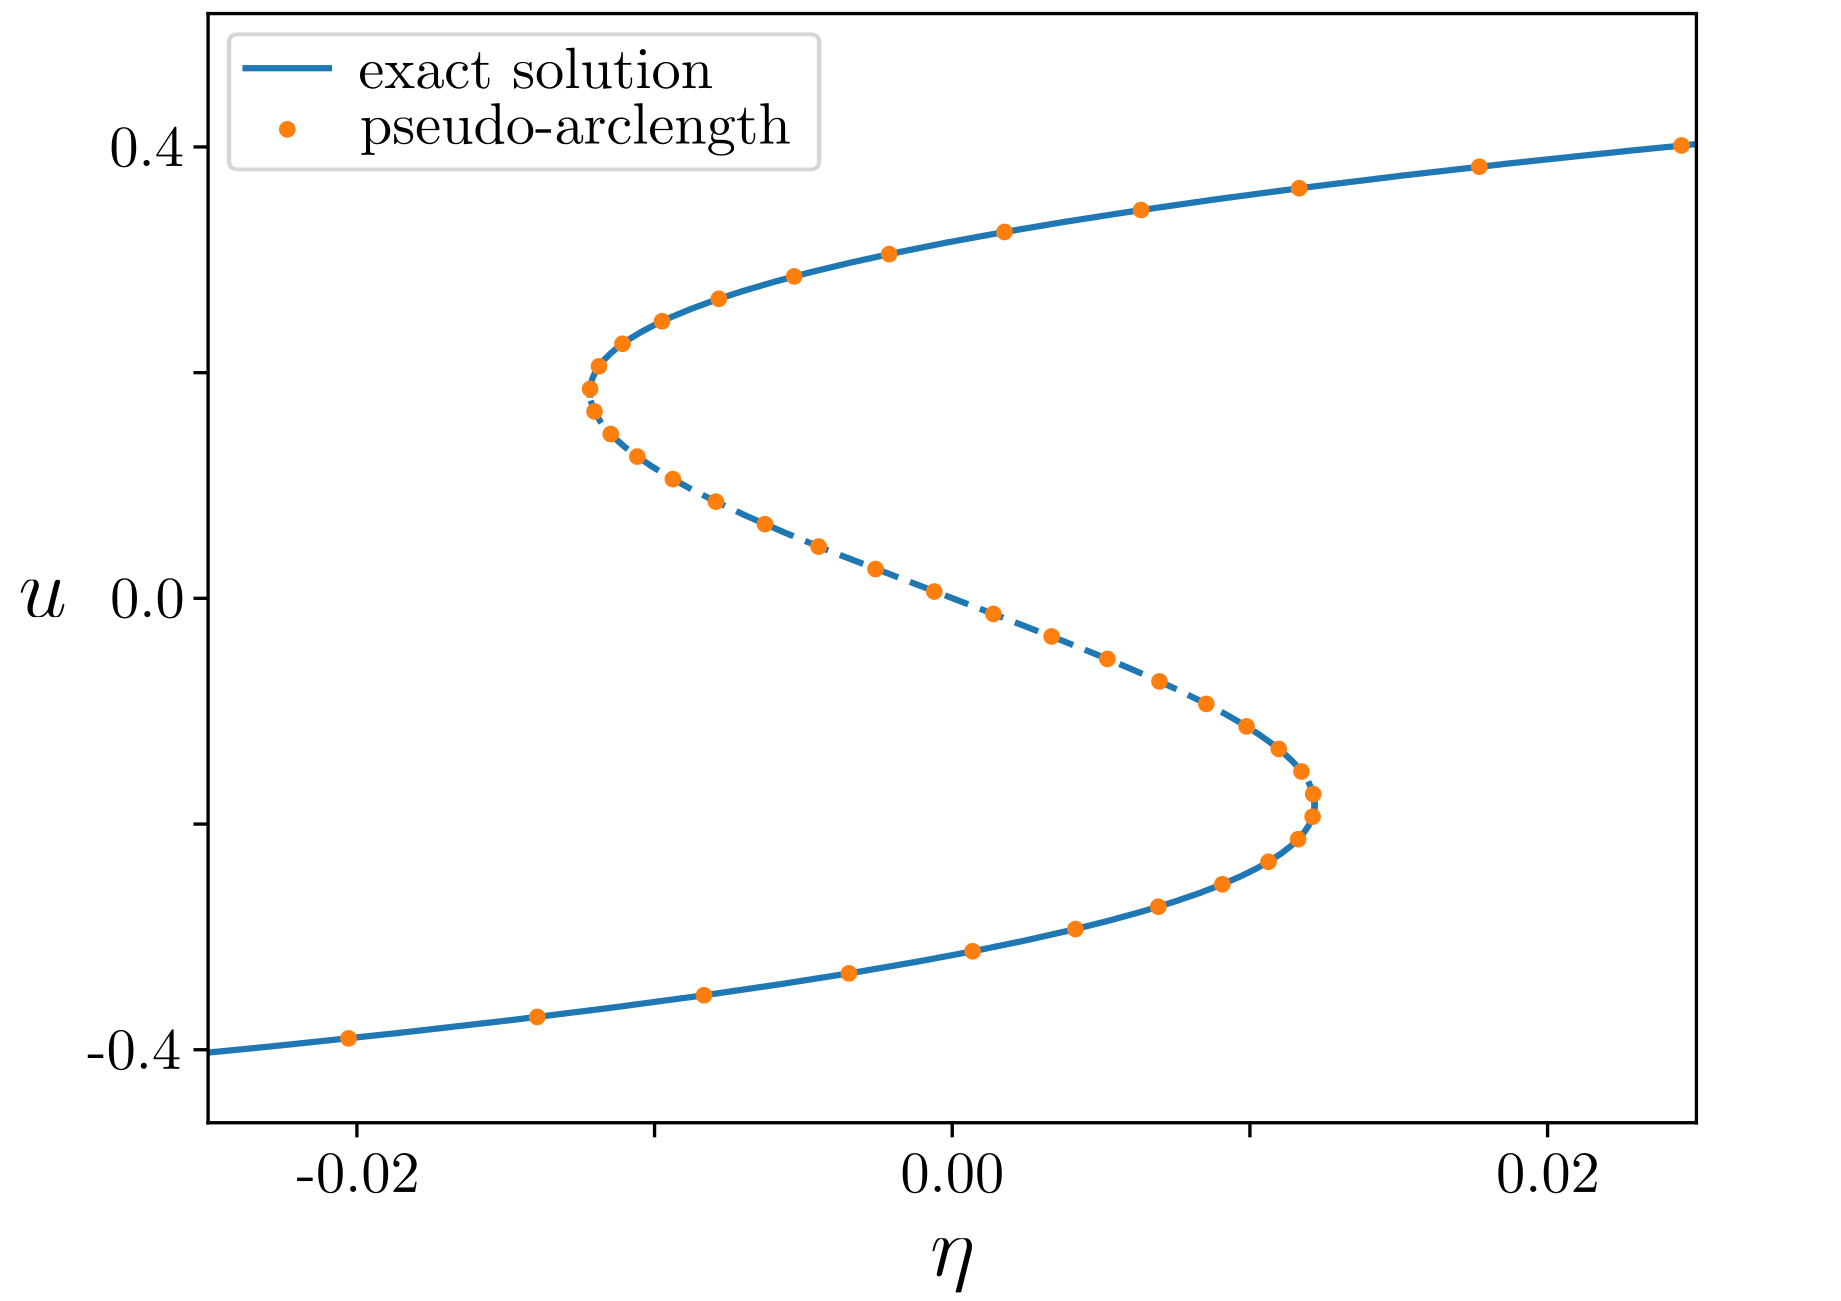
\includegraphics[width=0.7\textwidth]{scripts/figures/palc_she.png}
        \caption[short]{Solution of Eq.~(\ref{eq:pre_nc_palc_she}) as a function of the parameter $\eta$ obtained
        through the pseudo-arclength continuation (orange dots) compared to the exact solution (blue curve).}
        \label{fig:pre_nc_she}
        %\includesvg[width=0.5\textwidth]{scripts/figures/natural_continuation_she.svg}
    \end{figure}

\end{exmp}

\section{Continuation of traveling states}

In the particular case of following moving solutions with constant speed $c$, which is
the core of this work, some difficulties arise. The first and most evident one, is that
the desired solution is not steady anymore. This can be solved rather easily by
changing to the co-moving frame of reference, i.e. by inserting the traveling wave
ansatz $\bm{u}(x, t) = \bm{a}(x - ct)$, where $a$ is the solution profile in the co-moving frame,
 into Eq.~(\ref{eq:pre_nc_zeros}). Due to the chain rule,
an additional term in the form of a spatial derivative appears in the equation,

\begin{equation}
    0 = \bm{F}(\bm{a}, \eta) + c\partial_x\bm{a}
\end{equation}

The second problem is that usually the speed $c$ will change as parameters
are varied along the solution branch. Therefore, at
each step, the speed will have to be determined by the 
algorithm. The solution to this problem is to add the speed
as another unknown, that is to say, we will now be interested in solving for 
$\bm{y} = (\bm{a}, c, \eta)$. This leads to the third and final problem, which is that due
to the additional unknown, we are a missing an additional equation that will guarantee
a unique solution to the linearized system. Moreover, we will be solving these systems considering periodic
boundary conditions meaning that a translational invariance will appear. In order to
deal with the translational symmetry and guarantee a unique solution, a {\em phase condition}
or {\em pinning condition} must be established. Indeed, if we find a solution
$\bm{a}(x)$, then $\tilde{\bm{a}}_{\theta}(x) = \bm{a}(x  + \theta)$ is also
a solution for every $\theta$. 

The most widely used condition is the
{\em integral phase condition} \cite{doedel1981auto} which takes a reference solution $\bm{a}_0$ for a certain
parameter value $\eta_0$ close to the desired solution. The idea is to find the phase
that minimizes the difference $D$ between the desired solution $\bm{a}$ and the reference solution
$\bm{a}_0$. We can define the difference as follows,
\begin{equation}
    D(\theta) = \int_0^L dx' 
        \left|\left| \bm{a}(x' + \theta) - \bm{a}_0(x') \right|\right|^2    
\end{equation}

In order to minimize the difference, we differentiate the above equation, set it equal to zero and 
then integrate by parts. Thus, we arrive at the following condition which is simpler to
implement.

\begin{equation}
    p(\bm{a}, \bm{a}_0) = \int_0^L dx' \bm{a}(x') \cdot \left. \frac{d\bm{a}_0}{dx}\right\vert_{x'} = 0.
\end{equation}

We can re-define the extended vector function for which we want to find 
the root of in the following manner,

\begin{equation}
    \bm{H(\bm{y})} = \begin{pmatrix}
      \bm{F}(\bm{a}, \eta) + c\partial_x\bm{a} \\
    p(\bm{a}, \bm{a}_0) \\
    q(\bm{y}, \bm{y}_0)
    \end{pmatrix}
\end{equation}


The derivative of the integral phase condition with respect to the state vector $p_{\bm{a}}$ may differ depending on the chosen 
phase condition and implementation of the phase condition. In the simplest case, 
replacing the integral as a Riemann sum (which is the same as the trapezoidal rule in the case of periodic boundary conditions), the derivative reads

\begin{equation}
    p_{\bm{a}} = \Delta x \dfrac{d\bm{a}_0}{dx}.
\end{equation}

Therefore, the corresponding Jacobian of the extended function reads

\begin{equation}
    \matr{J_H}(\bm{y}) = \begin{pmatrix}
        \matr{J}(\bm{a}, \eta) + c\partial_x & \partial_x\bm{a} &  \bm{F}_\eta(\bm{a}, \eta)\\
        p_{\bm{a}}(\bm{a}_0) & 0 & 0 \\
        \dot{\bm{a}} & \dot{T} & \dot{\eta} \\
    \end{pmatrix}.
\end{equation}

Note that the last row corresponds, once again, exactly to the tangent vector
$\tau = (d\bm{u}/ds, dT/ds, d\eta/ds) = (\dot{\bm{u}}, \dot{T}, \dot{\eta})$.


\section{Continuation for periodic orbits}

If we know wish to follow periodic solutions with the continuation method we
must first derive a new set of equations to be solved. Mainly, periodic solutions
are not steady solutions of the differential equation, however they satisfy
the following boundary-value problem.

\begin{align}
    \dfrac{d\bm{u}}{dt} &= \bm{F}(\bm{u}, \eta) \\
    \bm{u}(t=0) &= \bm{u}(t=T)
\end{align}

It is convenient to rescale the time $t\to tT$, therefore the condition for
periodicity of the solution becomes $\bm{u}(t=0) = \bm{u}(t=1)$. Moreover,
due to the rescaling in time, a factor $T$ appears on the right-hand side of 
the dynamical equation. Therefore, the rescaled system becomes,

\begin{align}
    \dfrac{d\bm{u}}{dt} &= T\bm{F}(\bm{u}, \eta) \\
    \bm{u}(t=0) &= \bm{u}(t=1)
\end{align}

Moreover, due to the additional time-dependence of $\bm{u}$, the parametrizing equation for the pseudo-arclength
method needs to be modified accordingly. It now reads,

\begin{equation}
    q(\bm{y}, \bm{y}_0) = \int_0^1  (\bm{u}(t) -  \bm{u}_0(t)) \cdot \dfrac{d\bm{u}}{ds} dt 
        + (T - T_0) \dfrac{dT}{ds} + (\eta - \eta_0) \dfrac{d\eta}{ds} - \Delta s = 0 
\end{equation}

Additionally, one can add weights to the
previous equation in order to tune the search direction in Newton's method "horizontally"
(taking larger steps in the parameter $\eta$) or "vertically" (smaller steps in $\eta$),
see \cite{Uecker2017pde2path} for a more detailed discussion.

Note that we have introduced the period $T$ as another unknown which will be solved
through Newton's method along with $\bm{u}$ and $\eta$, i.e. we want to solve
for $\bm{y}(t) \equiv (\bm{u}(t), T, \eta)$. Moreover, as in the previous section, a phase condition
$p(\bm{u}, \bm{u_0}) = 0$ must be satisfied in order to deal with the translational invariance (in time) and
guarantee the uniqueness of the solution.
Finally, we can re-define the
extended vector function for which we want to find the root of in the following manner,

\begin{equation}
    \bm{H(\bm{y})} = \begin{pmatrix}
       T \bm{F}(\bm{u}, \eta) - \frac{d\bm{u}}{dt} \\
    p(\bm{u}, \bm{u}_0) \\
    q(\bm{y}, \bm{y}_0)
    \end{pmatrix}
\end{equation}


In order to solve this system of equations subject to periodic boundary conditions, many strategies can be followed. Namely, orthogonal collocation methods
(implemented in AUTO \cite{doedel1981auto}), multiple shooting methods \cite{keller1968numerical}, and last but not least, finite difference methods
(implemented in pde2path \cite{Uecker2017pde2path}). Although the latter has the least accuracy it is by far the 
simplest to implement. In the finite difference method, a possible approximation to the
first equation in the above system is the trapezoidal rule (used for instance in the Crank-Nicolson
scheme for simulating PDEs),

\begin{equation}
    \left( \dfrac{F(\bm{u}_i) + F(\bm{u}_{i+1})}{2} \right) T 
        - \dfrac{\bm{u}_{i+1} - \bm{u}_{i}}{t_{i+1} - t_i} = 0
\end{equation}

Note that the derivative of $\bm{u}$ with respect to $t$ can be written as a product
of a matrix $\matr{\nabla}_t$ and the time-discretized vector $\bm{u}_i$ $(1 \leq i \leq n_t)$, i.e.
it can be written as $\matr{\nabla}_t\bm{u}$, in which case the Jacobian $\matr{J_H}$ of $\bm{H}$
reads

\begin{equation}
    \matr{J_H}(\bm{y}) = \begin{pmatrix}
        T \matr{J}(\bm{u}, \eta) - \matr{\nabla}_t & \bm{F}(\bm{u}, \eta) &  T\bm{F}_\eta(\bm{u}, \eta)\\
        p_{\bm{u}}(\bm{u}_0) & 0 & 0 \\
        \dot{\bm{u}} & \dot{T} & \dot{\eta} \\
    \end{pmatrix}.
\end{equation}


\chapter{Isolas of localized structures and Raman–Kerr frequency combs in micro-structured resonators (Chaos, Solitons \& Fractals 174, 113808)}

In section~\ref{sec:fra_LS} the concept of dissipative 
localized structures (LSs) was introduced. These states can be observed in a huge variety
of systems including vegetation patterns, biology and 
nonlinear optics \cite{tlidi2014localized,heimburg2005soliton}. In the case of nonlinear optical systems,
a particularly interesting type of localized structure can be identified,
the so-called optical solitons. Moreover, it has recently been discovered that the formation of solitons
in both fiber and micro-resonators gives rise to frequency combs, which are equally
spaced spectral lines. These frequency combs are exceedingly useful
for technological purposes such as chip-scale atomic clocks \cite{Jost2015clock}, terabit
per second communication \cite{marin2017microresonator} and even the calibration of spectrometers
for exoplanet search \cite{suh2019searching}. From a theoretical perspective, the dynamics
of solitons in these optical resonator systems can be accurately described 
by the paradigmatic Lugiato-Lefever equation (LLE) \cite{lugiatolefever1987}.

The aim of this chapter is the study of the formation of such structures in the
case of short solitons where the influence of the stimulated Raman scattering (SRS)
cannot be neglected and higher-order dispersion terms appear. In this case, a reduced model
in the form of a non-local Swift-Hohenberg equation is proposed to provide 
analytical results and an in-depth numerical description. By means of a combination of
numerical simulations and
continuation of the reduced model (see \ref{sec:cont_traveling} for a detailed discussion on the
continuation of traveling states), it can be seen that the SRS induces a forced symmetry
breaking leading to the motion of both the bright and dark solitons, as well as a disconnection between 
the different branches of LSs. Consequently, the traditional snaking bifurcation scenario breaks
apart and instead, a family of isolas emerges. Lastly, a numerical analysis of the
original model, the generalized LLE, confirms both the formation of drifting LSs and
the presence of isolas due to the reflection symmetry breaking, in agreement with previous studies \cite{burke2009swift,parra2014third}.

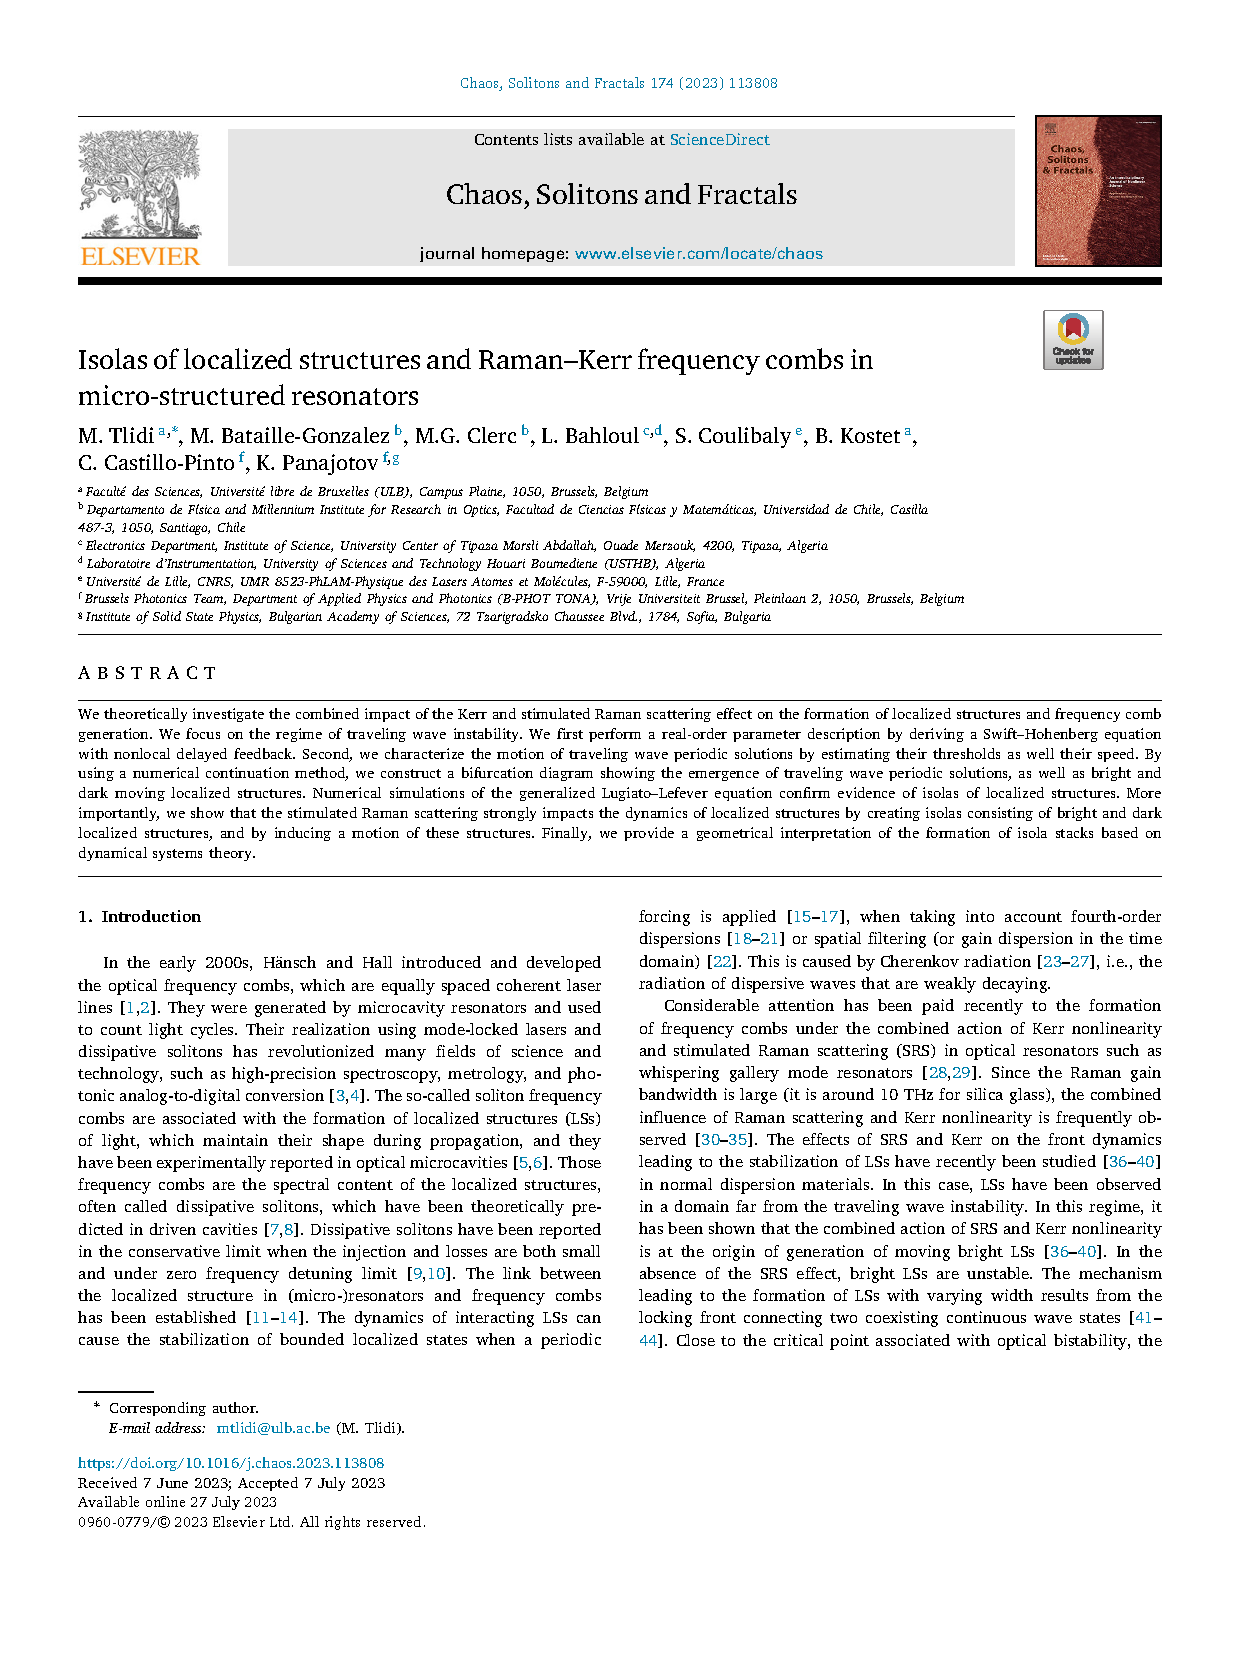
\includepdf[pages={-}]{chapters/isolas.pdf}

\section{Perspectives}

In this work, we have performed a detailed numerical analysis of the formation
of bright and dark solitons in a reduced non-local Swift-Hohenberg equation. More specifically,
the effect of a reflection symmetry-breaking term was investigated: the Raman effect on 
the LSs. Additionally, these results have been represented in a 
detailed bifurcation diagram. 
Nevertheless, not all of the bifurcations
present in the diagram were completely characterized.
For instance, the traveling 
wave and most LSs lose stability before the saddle-node bifurcation at an unidentified
bifurcation point. Thus, further work is needed in this direction.
 On the other hand, although the main results have been successfully
confirmed on the original model, a more complete bifurcation diagram, showing the stability and all of the LSs, 
remains
to be produced.


\chapter{Dissipative Soliton Combs with Spectral Filtering. (submitted to IEEE Journal of Quantum Electronics)}

The previous chapter focused on the formation of dissipative solitons in optical
resonators when a non-local term due to Raman scattering is incorporated into the Lugiato-Lefever equation. The
integral form of this additional term poses several analytical and numerical difficulties.
For instance, in the case of the numerical continuation, where a
large system of equations needs to be solved, the addition of the integral term transforms the extremely sparse
system into a dense system, increasing the computational cost in terms of both memory and time
by orders of magnitude.

An alternative approach to deal with the integral form of a non-local operator is to represent
it by an infinite Taylor series, also referred to as a gradient expansion \cite{murray2003mathematical}. Moreover, 
assuming that the kernel function is sufficiently localized, the expansion can be
safely truncated and only the first few relevant terms can be kept. This way, the integral operator can be
approximated by a few differential operators with coefficients that depend on
the kernel. Consequently, the representation in terms of differential operators
allows for a much easier analytical investigation and numerical characterization of the system.
For this reason, this gradient approximation to a nonlocal operator has been widely 
preferred in studies of vegetation patterns \cite{lefever1997origin,clerc2021localised,pinto2022vegetation,pinto2023topological}.

In what follows, we apply the alternative approach stated above to investigate
the formation of solitons and patterns in a fiber ring resonator with a spectral filter.
To justify the use of a truncated gradient expansion, the case of a large-bandwidth filter
(or equivalently, a localized temporal filter) is considered. Starting from an infinite-dimensional
Ikeda map, a partial differential equation is derived in the form of a Lugiato-Lefever equation with additional
first and second derivative terms from the gradient approximation. Similarly, as in the previous chapter,
a forced reflection symmetry breaking takes place, leading to the drift of both localized and periodic states.
Furthermore, it is observed that, in the presence of the filter, the stability region of LSs is significantly reduced
and, the Andronov-Hopf bifurcation point that gives rise to breathing solitons is shifted towards a larger pumping.
Lastly, through numerical continuation, the persistence of the snaking bifurcation scenario in
the presence of the diffusive term is revealed along with its destruction upon the addition of the reflection symmetry-breaking term.

\includepdf[pages={-}]{chapters/filtering.pdf}

\section{Perspectives}

In this article, we showed that, under the addition of a spectral filter, a series of
derivative terms must be incorporated into the LLE. Then, assuming a sufficiently
localized filter, we justified a second-order truncation of the series and studied 
the effects of the additional terms with coefficients $\alpha_1, \alpha_2$ on the stability and dynamics of both localized 
and periodic structures. However, a more extensive exploration of the system's parameters 
remains to be performed. In this direction, a phase diagram showing the stability boundaries
in terms of these two coefficients would provide a more complete description and be
especially helpful for experimentalists. On this note, it would also be interesting to
compute the coefficients corresponding to previous experimental studies \cite{bessin2019gain}
and test whether our approximation is still valid in a real experiment. If this is not the case,
then a detailed numerical analysis via continuation of the integrodifferential 
equation deserves to be performed and compared with the results shown in this chapter.


%\chapter{Moving Solitons in the Lugiato-Lefever equation.}

In section~\ref{sec:fra_LS} we introduced the concept of dissipative localized structures (LSs). Here, we will study the formation
of such structures in nonlinear optical systems where they are often called optical or cavity solitons. 
More specifically, we will analyze the paradigmatic Lugiato-Lefever equation (LLE) \cite{lugiatolefever1987} used to describe fiber resonators, and
study the formation of LSs when a fourth order derivative and a non-local term are considered.


\section{Lugiato-Lefever equation.}

In 1987, Lugiato and Lefever proposed a simple yet extremely rich nonlinear partial differential equation to study the formation of patterns and localized states
in the framework of nonlinear optics \cite{lugiatolefever1987}. They considered a cavity filled with a nonlinear medium in the low transmission (or high quality) limit
driven by a continuous wave. In order to keep the equation as simple as possible, they considered a cubic nonlinearity which is characteristic of Kerr media. Moreover,
In virtue of the low dissipation limit, they originally neglected the longitudinal variable $z$ (along which light propagates) and kept only the transversal plane $x-y$ as spatial
variables in the equation. In contrast, a longitudinal (or temporal) LLE was later formulated by Haelterman and his colleagues [ref], where only the longitudinal 
coordinate becomes relevant. The main difference between these two equations is that in the former, a transversal Laplacian appears due to diffraction of the light, whereas
in the latter, a longitudinal Laplacian appears due to dispersion of the light. However, from a mathematical point of view, they are the same equations.


\begin{equation}
    \dfrac{\partial E}{\partial t} = E_{in} - (1 + i\theta) E + i |E|^2 E + i\nabla^2 E
    \label{lle:lle}
\end{equation}

In our case, we will consider the longitudinal LLE corresponding to Eq.~(\ref{lle:lle}) as a starting point and we will analyze
the effect of adding a fourth order dispersion term and the Raman effect which will be explained in the following section.

\section{Raman effect.}

Raman effect frequently observed 26-31. 

Stabilization of LSs by means of the Raman effect. 39, 41, 41-43 in normal dispersion and far from MI. 

\section{Isolas and traveling solitons.}

In that case the LS is formed due to front locking between the two CW solutions (i.e. it requires bistability). 
However, in this case the LS arise due to coexistence between periodic state and CW, so even in the monostable can be observed.

\begin{SCfigure}
    \centering
    \caption{asdasd}
    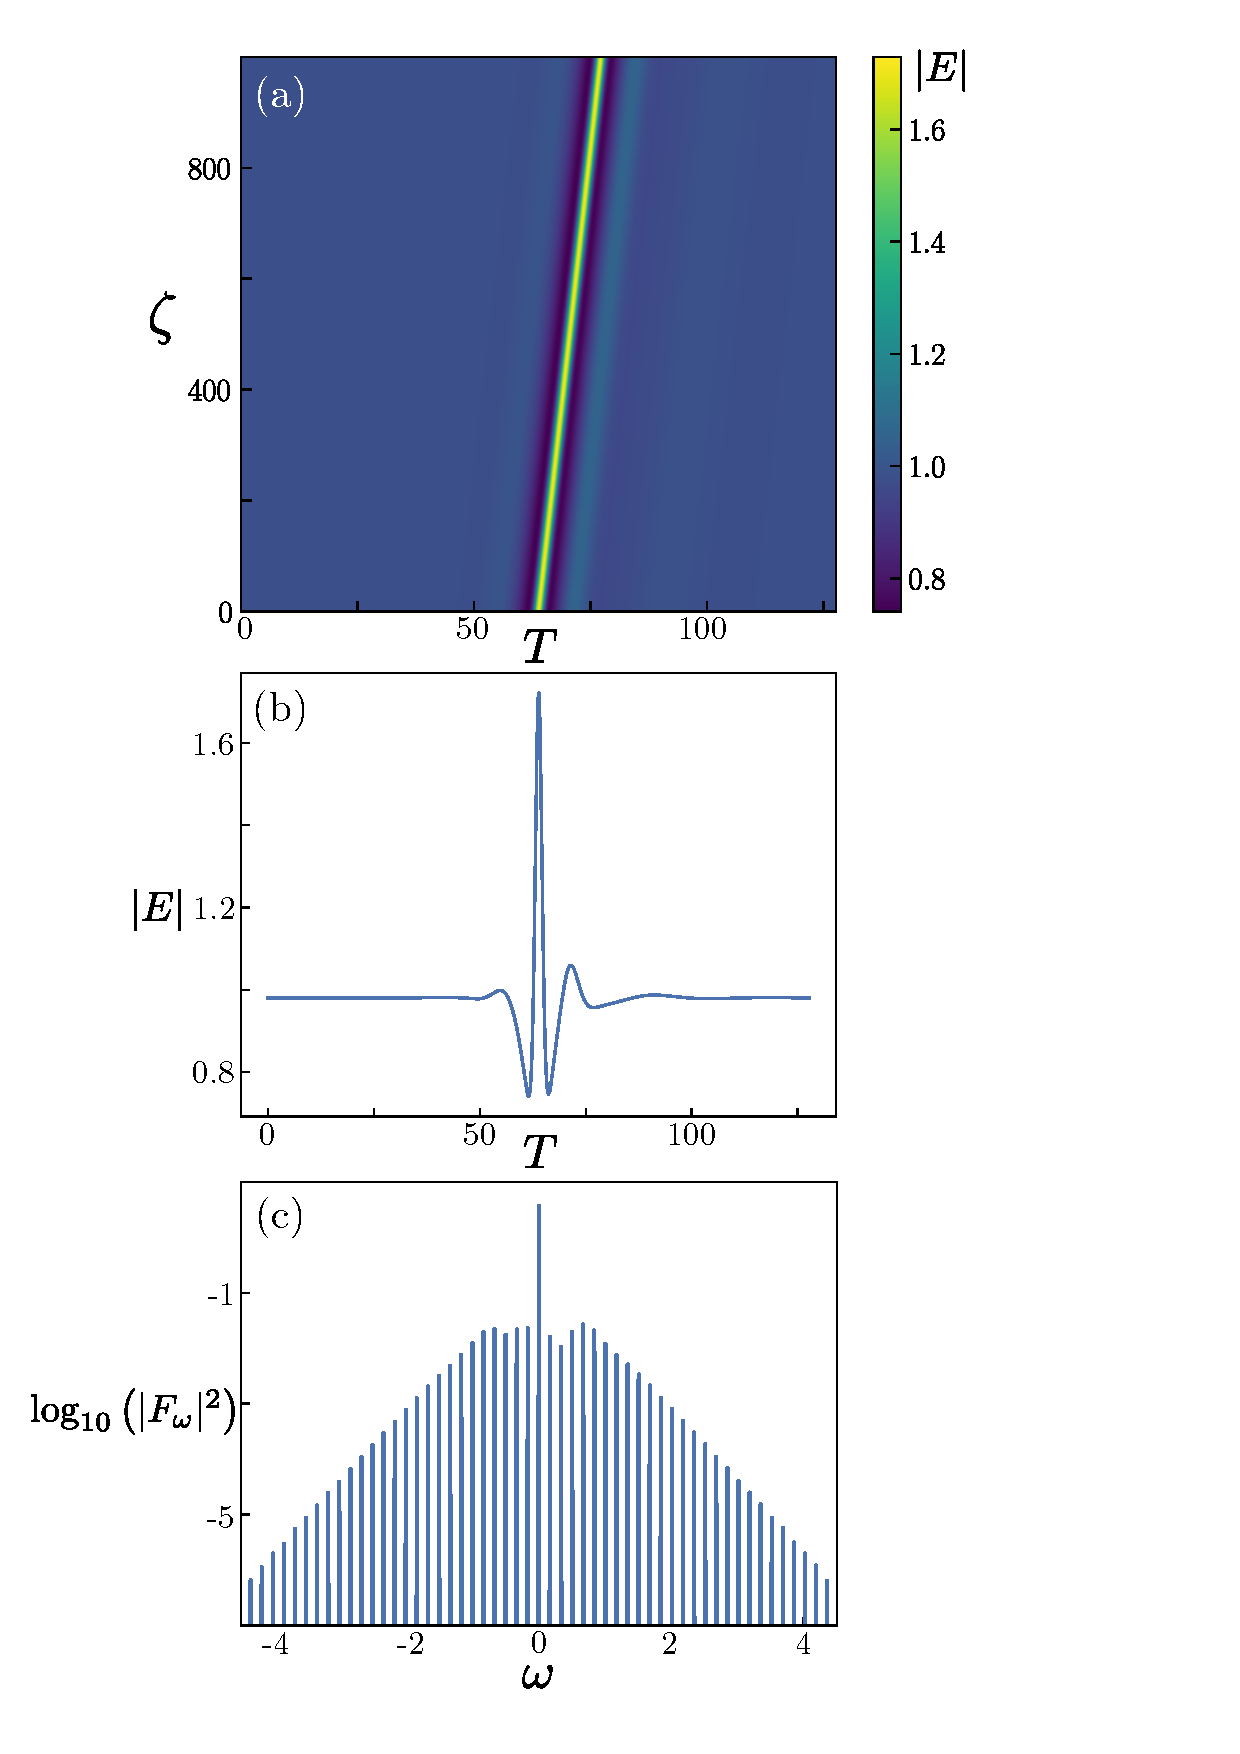
\includegraphics[width=0.6\textwidth]{imagenes/lle/LLE_Spatiotemporal.pdf}
\end{SCfigure}

\begin{figure}
    \centering
    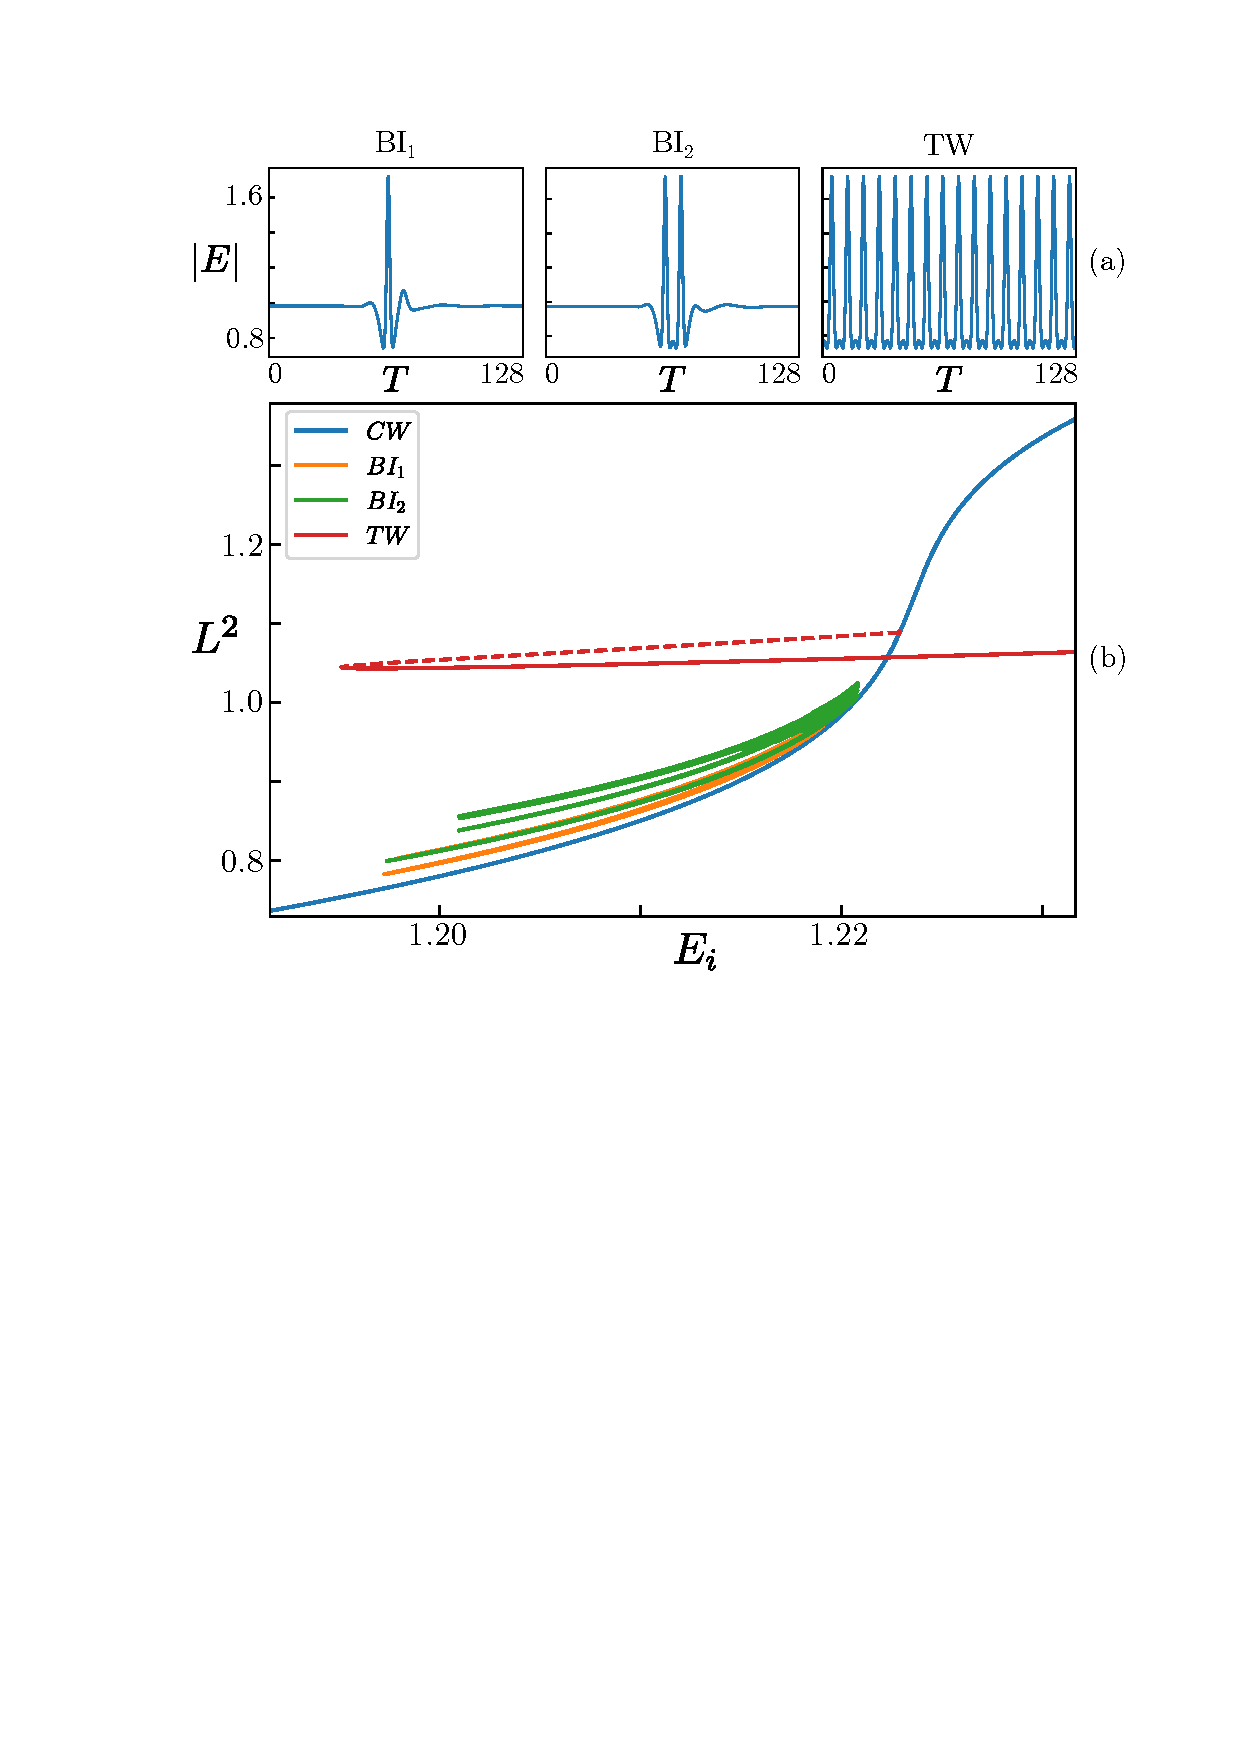
\includegraphics[width=0.7\textwidth]{imagenes/lle/LLE_Isola.pdf}
    \caption{asd}
\end{figure}

\section{A reduced model.}

\begin{SCfigure}
    \centering
    \caption{asdasd}
    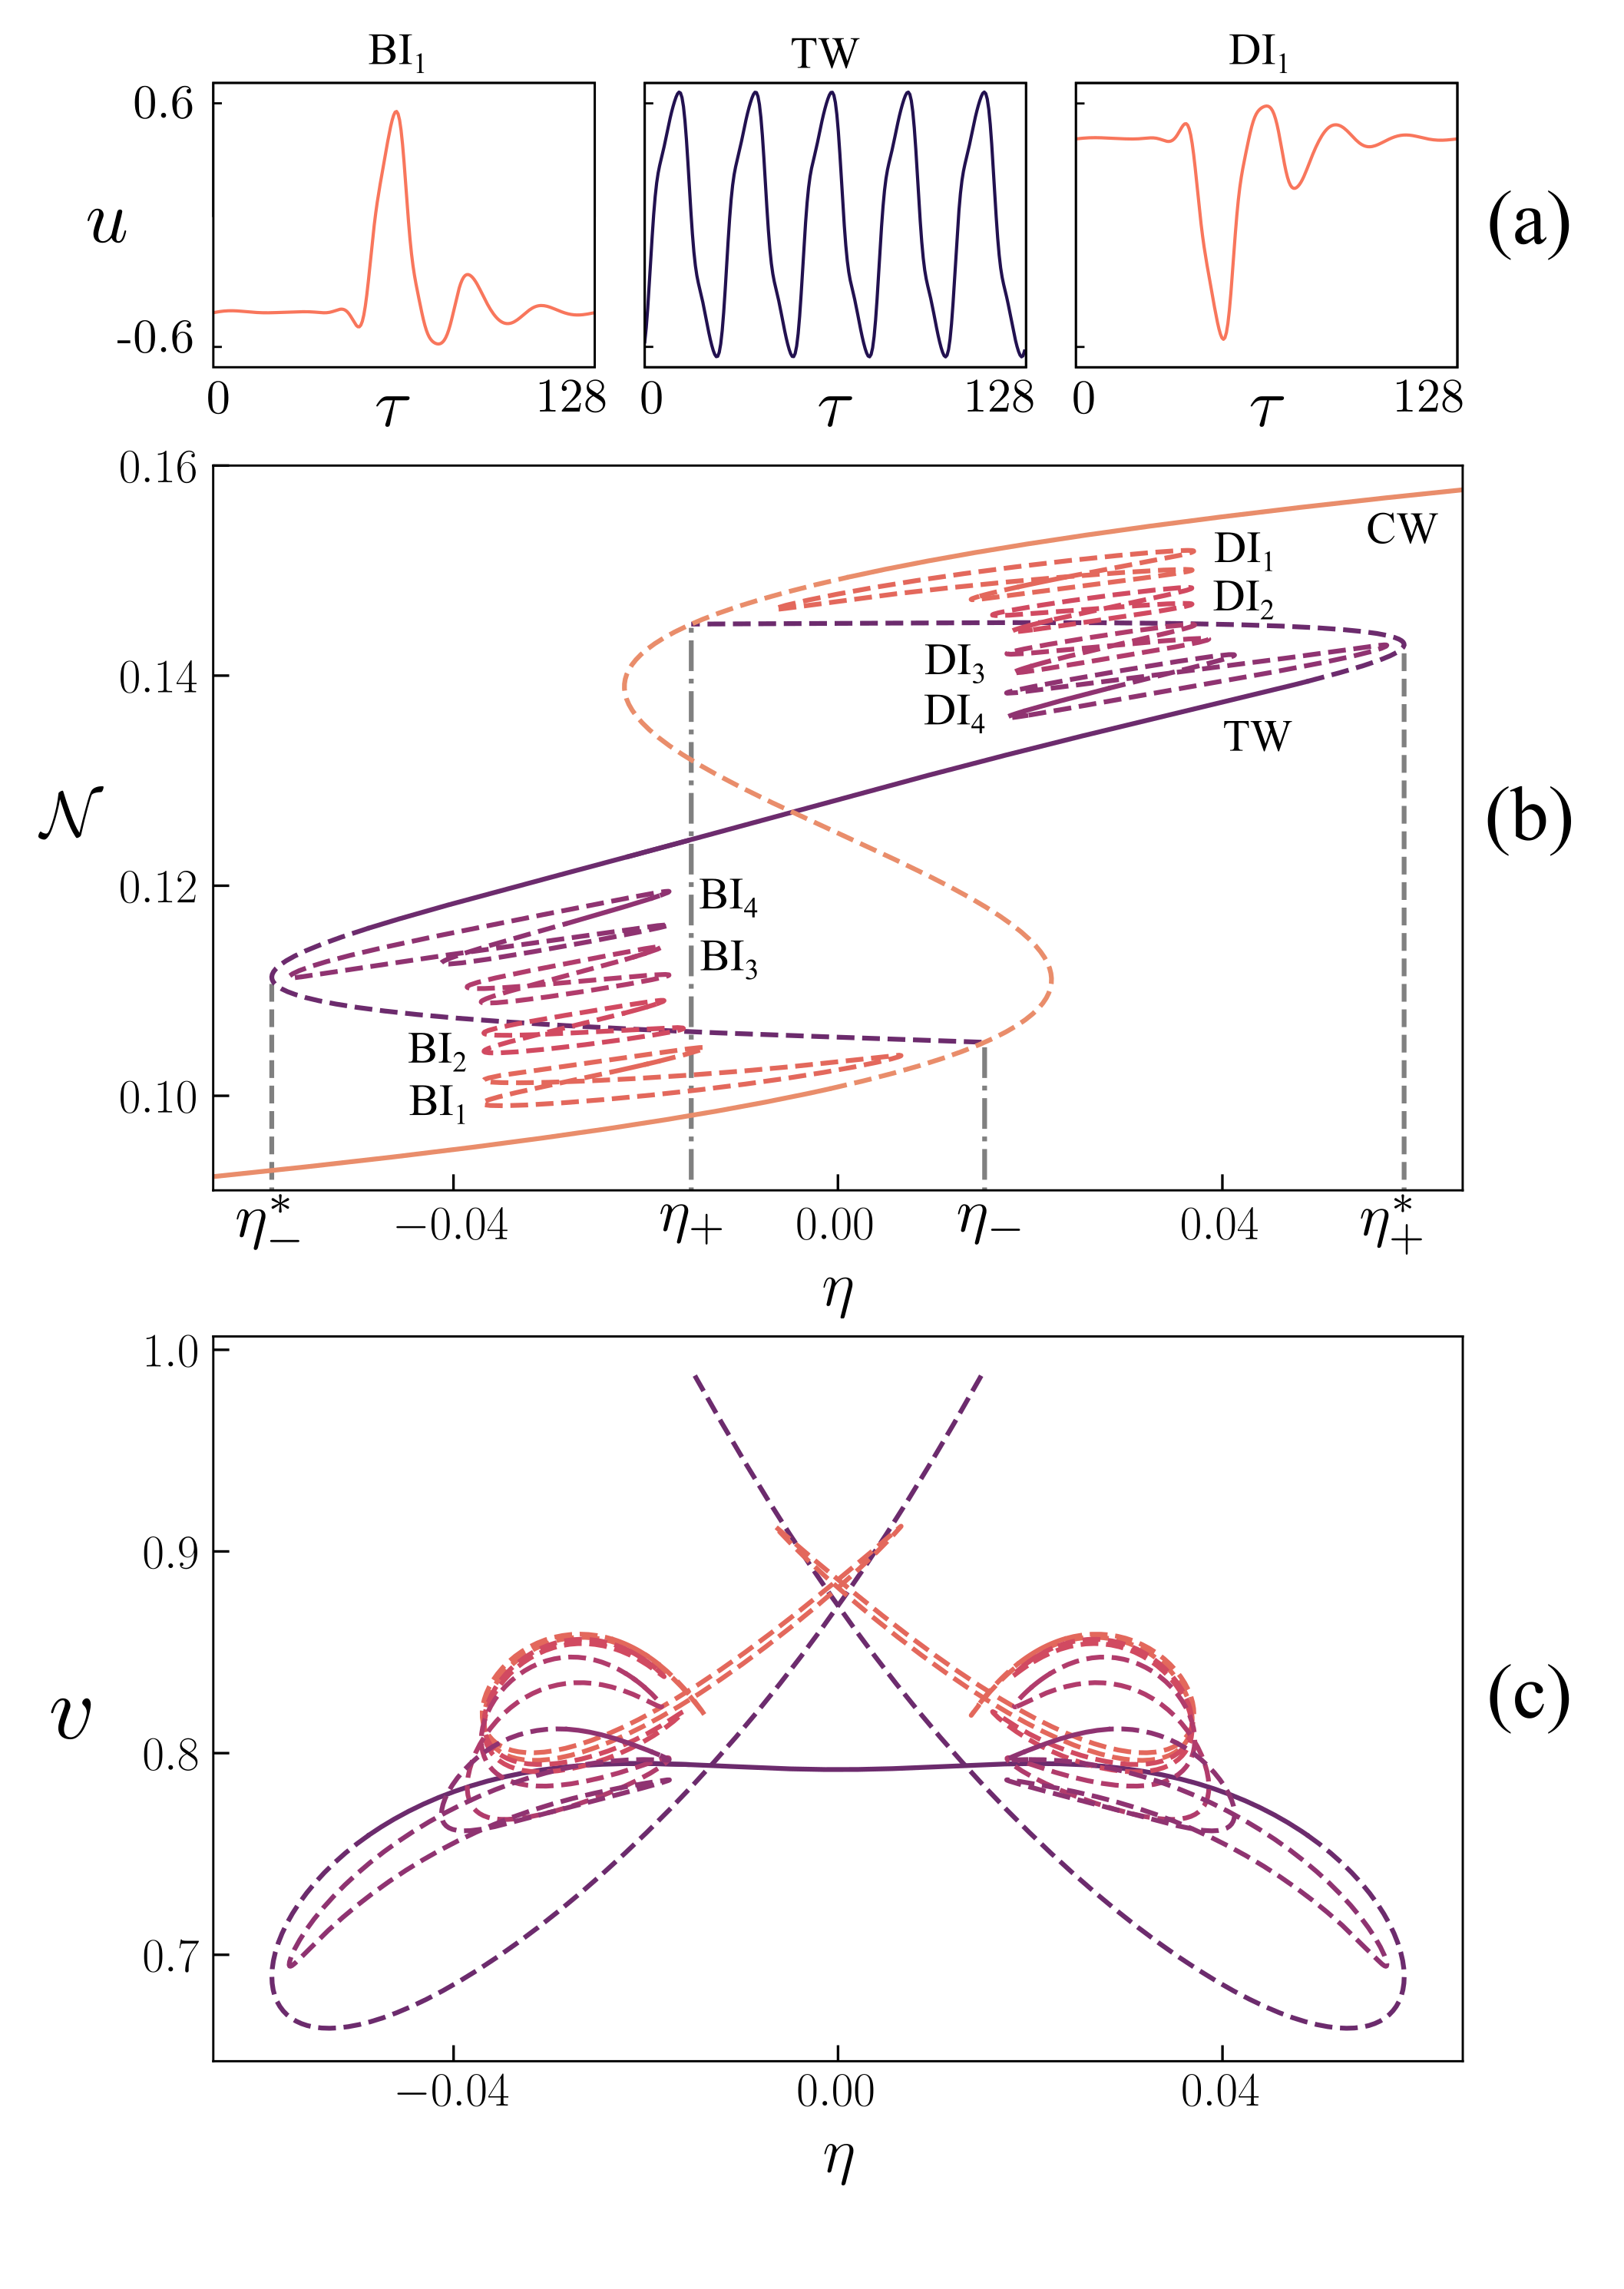
\includegraphics[width=0.6\textwidth]{imagenes/lle/Fig3.png}
\end{SCfigure}

\begin{figure}[h]
    \centering
    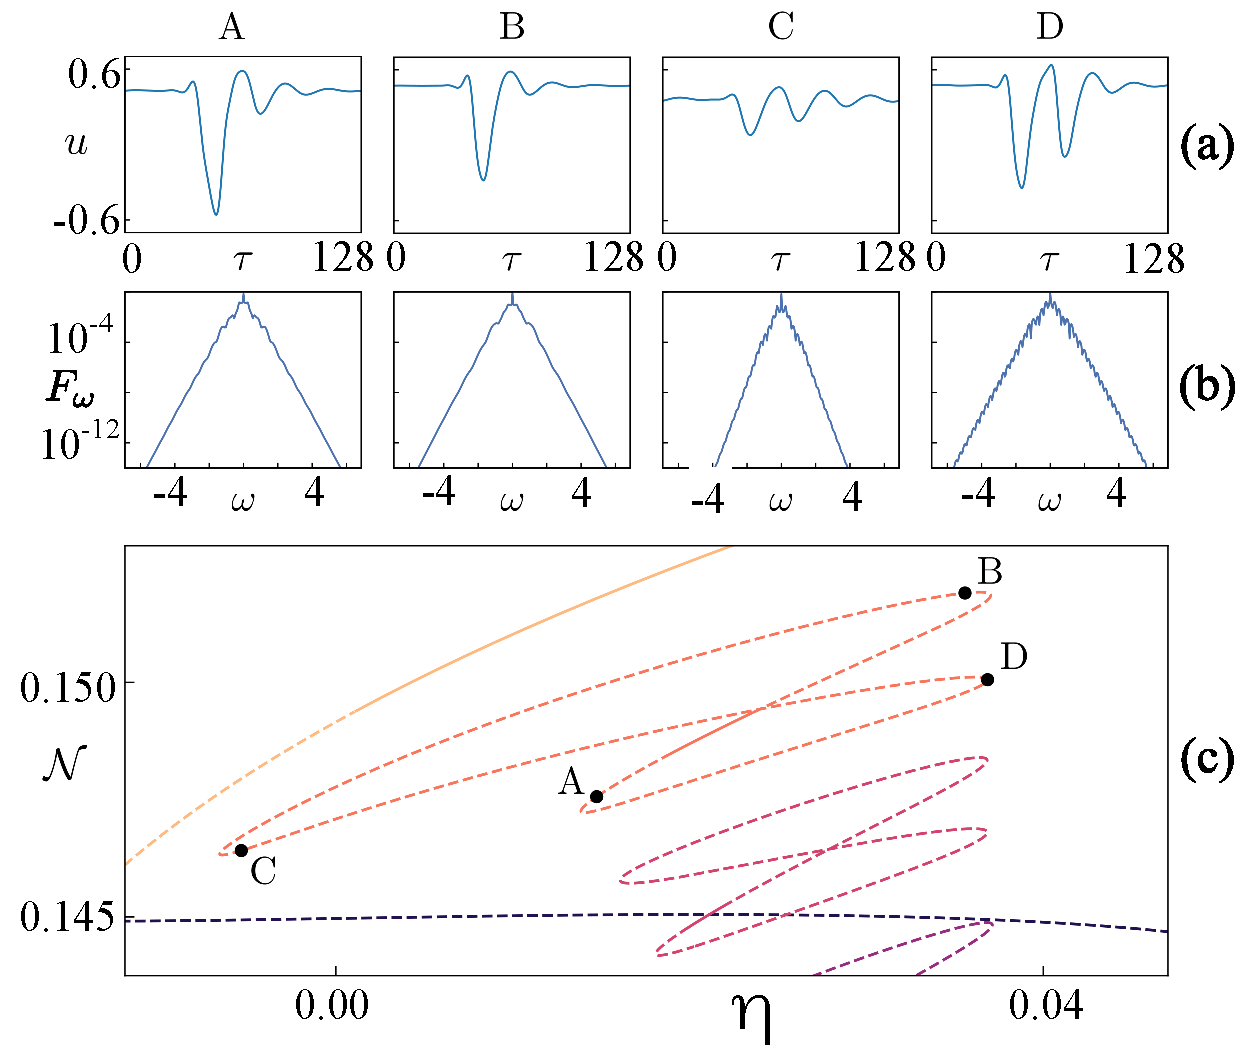
\includegraphics[width=0.5\textwidth]{imagenes/lle/Fig4-Isola.pdf}
    \caption{asd}
\end{figure}

\section{Oscillatory bound states.}

\begin{enumerate}
    \item 
\end{enumerate}
\chapter{Moving spiral wave chimeras (Physical Review E, 104(2), L022203)}

So far, this investigation has focused on drifting one-dimensional localized states in
two non-local optical systems. 
In these two cases, the motion itself was expected since a reflection
symmetry-breaking term was present. Nevertheless, such a term is not always
necessary to set localized states in motion. Indeed, this chapter exposes that motion can arise spontaneously
in an isotropic system of coupled phase oscillators.

In section~\ref{sec:phase_oscillators}, the importance
and universality of phase oscillators have been emphasized, as they offer a comprehensive
description of self-sustained oscillators at the cost of neglecting the amplitude 
dynamics. Such oscillators are ubiquitous, they can be found in flashing fireflies, lasers, neurons, and even pacemaker cells in the heart.
The dynamics of an individual oscillator is already a challenging research problem, as evidenced
by the Nobel Prize awarded to Hodgkin and Huxley for their neuron model
\cite{hodgkin1952quantitative}.
Furthermore, the dynamics of a population of coupled phase oscillators
offers even greater complexity and richness. A fundamental question that
arises in these interacting oscillators systems is whether they will synchronize, 
and if so, to what degree.

While numerous authors have made tremendous advances on this topic [citas], one of the
most outstanding is Kuramoto who provided a simple yet powerful model 
for describing coupled oscillators several decades ago \cite{kuramoto1975model}. 
Even nowadays, the Kuramoto
model and its modifications remain a very active research field [citas].
Remarkably, when Kuramoto and Battogtokh extended the model considering non-local coupling instead
of the original global coupling, they observed an incongruous state
of partial synchrony where coherent (synchronized) and incoherent (desynchronized) domains coexisted \cite{kuramoto2002coexistence}.
It could be expected that coupling identical oscillators would only yield a completely coherent
state, yet they showed that the symmetry could be spontaneously broken and the system
would self-organize into two different and coexisting domains, what we now call a chimera state \cite{abrams2004chimera}.

Even more surprisingly, two-dimensional simulations of the Kuramoto-Battogtokh model
revealed a planar chimera state in the form of a spiral wave. This spiral wave chimera
presented an incoherent core at the tip of the spiral where oscillators were desynchronized
while the remaining oscillators located in the spiral arms were synchronized. Similar spiral
patterns had already been observed in reaction-diffusion systems except for one significant
difference; the phase singularity located in the tip of the spiral was now replaced by
an incoherent core. Since then, spiral chimeras have been repeatedly observed both numerically [citas] and experimentally [citas]
in a variety of systems. 

In this chapter, we investigate the dynamics of a bound state of two counter-rotating spiral wave chimeras
 in a two-dimensional array of coupled non-identical
phase oscillators. To eliminate the finite-size noise, the
continuum limit of infinitely many oscillators is studied in detail
by numerically simulating the
associated Ott-Antonsen equation. Although a symmetric and isotropic coupling function is considered,
the top-hat function, a spontaneous symmetry breaking arises which causes
the two-core spiral chimeras to develop a permanent motion. Consequently,
the formation of a crescent-shaped filamentary pattern is observed in the incoherent core
of the spirals, and is oriented towards the direction of motion.  Moreover, 3 
different two-core spiral chimeras are identified according to their motion, namely symmetric, asymmetric
and meandering spirals, and determine their stability region.

% Sacar we, occur, one would think, no but, so , also, 
% pasado y presente perfecto.

% 2d extension: spiral wave chimera. similar to spiral wave, experiments, relevance
 
% in this chapter
% importance of synchronization. 
% synchronization: Huygens (history), Kuramoto (predictions, see section xx).
% one could expect they synchronize but chimera state! kuramoto battogtokh,
% experiments, etc. introduce spiral wave chimera

% in this chapter...

% Coupled oscillators, synchronization. Very important in many contexts, brain, heart,
% power grid, etc.

% Unexpectedly, a different state was also found: the chimera state. explain
% They have been predicted and experimentally observed in a plethora of systems
% [refs]. 

% In the weak coupling limit, these populations of nonlinear oscillators can be accurately
% described by a simple yet powerful model: the Kuramoto model. 


% This second half will be devoted to the study of coupled phase oscillators. As
% stated previously, in section~\ref{sec:phase_oscillators}, the dynamics of
% a non-linear oscillator, in the limit of weak coupling, can be reduced
% to a single cyclic variable: the phase. Therefore, an adequate and general model
% for a population of coupled oscillators  

% [synchronization in the brain] \cite{erra2017neuralsynchronization}

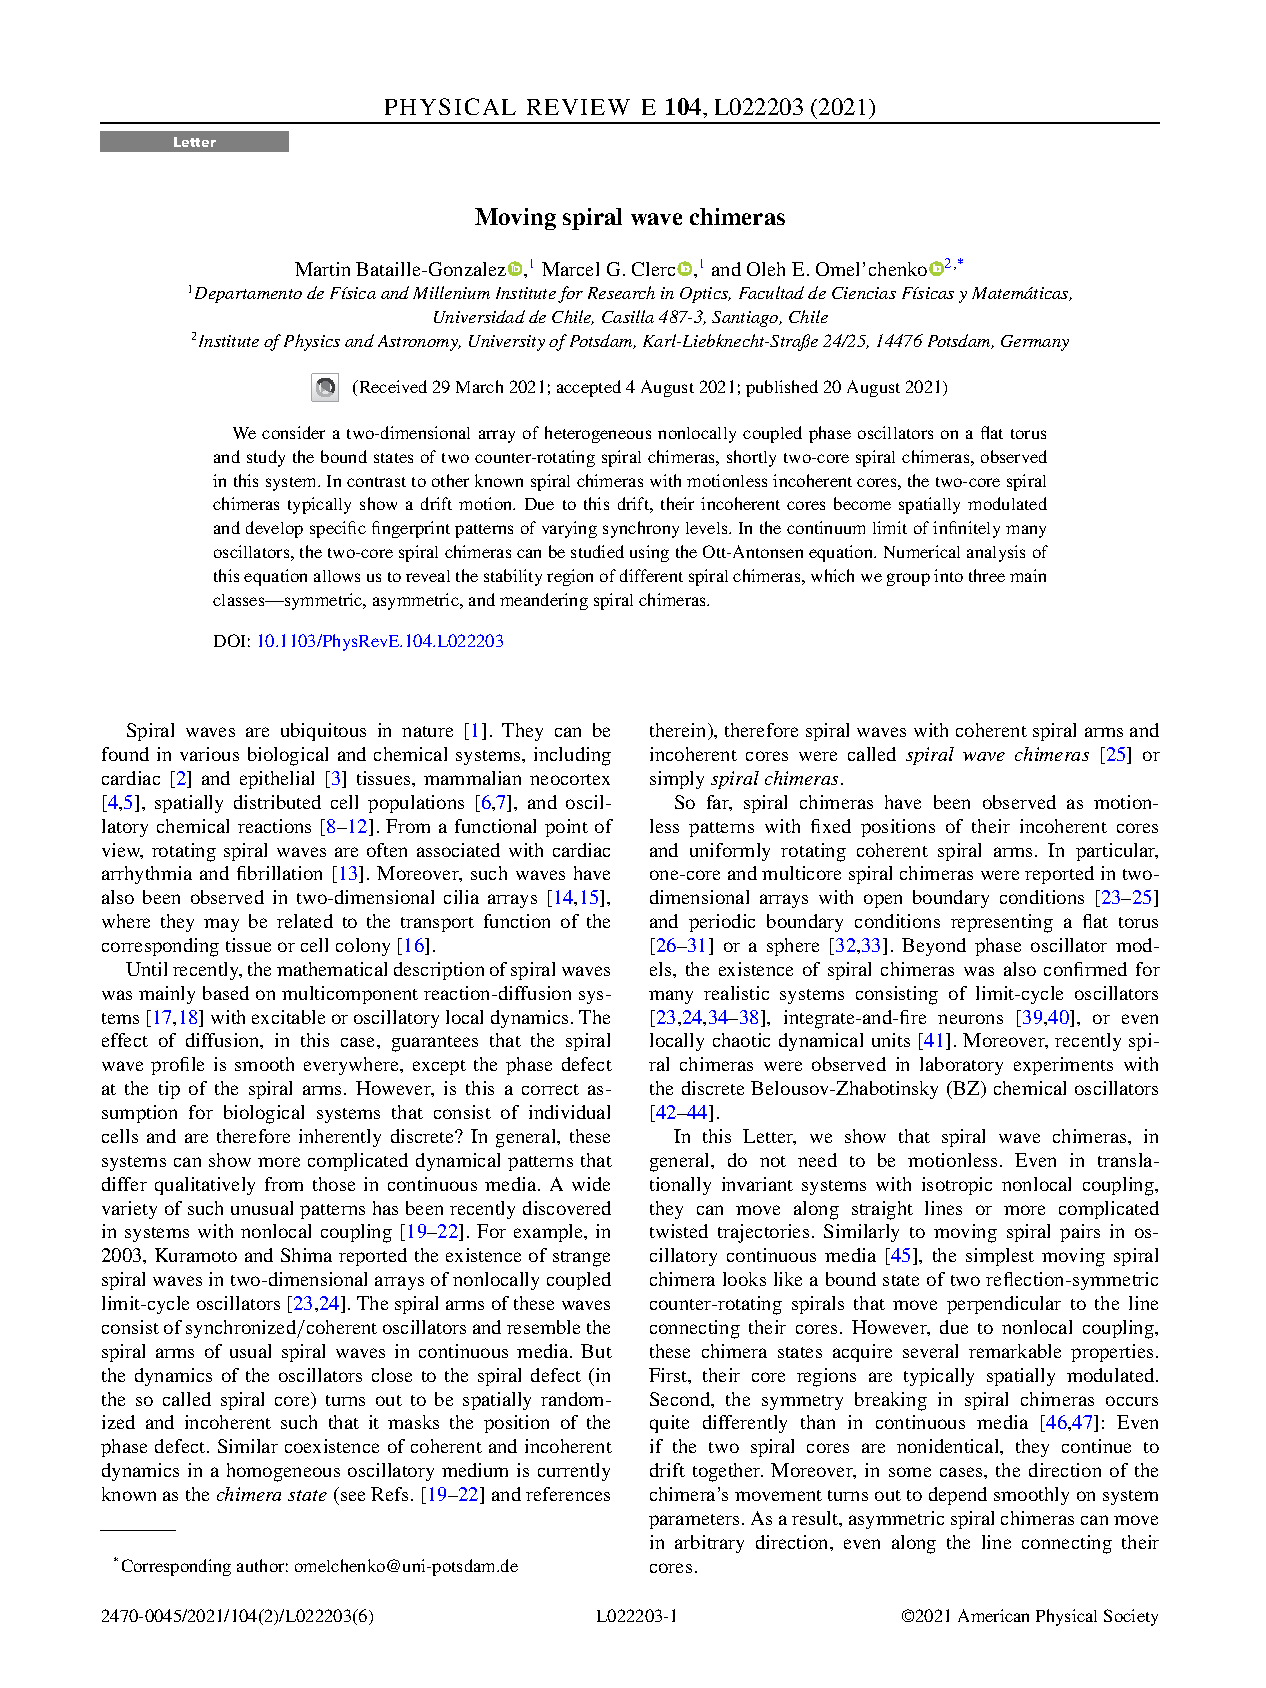
\includepdf[pages={-}]{chapters/movingspirals.pdf}

\section{Perspectives}
 

In this work, we have shown that even in a symmetric system, two-core
spiral chimeras move in three different ways. Furthermore, the stability region of symmetric, 
asymmetric and meandering spirals has been identified and presented in a phase diagram.
Nevertheless, a more in-depth numerical analysis is still needed to find not only
stable but also unstable states. This information will be fundamental to indentify
the various bifurcations that lead to the emergence of two-core spiral chimeras
from a homogeneous state, as well as the transition between symmetric and asymmetric
spirals. On the other hand, we have examined the effect of a top-hat coupling function
which has numerical advantages but may not be experimentally relevant. Therefore,
the extent to which these results apply to more realistic couplings remains
to be determined.

\chapter{Traveling spiral wave chimeras in coupled
oscillator systems: emergence, dynamics, and
transitions (New Journal of Physics 25, 103023)}

\includepdf[pages={2-}]{chapters/travelingspirals.pdf}

\section{Perspectives}


\chapter{Conclusions}

\lipsum[130-132]
\begin{figure}
	\centering
	
\includegraphics[scale=.2]{imagenes/fcfm.pdf}
	\caption{Logo de la Facultad}
	\label{logofcfm}
\end{figure}

\lipsum[133-134]

\begin{table}
	\centering
	\caption{Tabla 1}
	\label{tabla:1}
	\begin{tabular}{|c|c|r|}
		\hline
		\textbf{Campo 1} & \textbf{Campo 2} & \textbf{Num} \\\hline
		Valor 1a & Valor 2a & 3\\
		Valor 1b & Valor 2b & 3\\
		\hline
	\end{tabular}

\end{table}

\lipsum[135]


% ver https://www.overleaf.com/learn/latex/Glossaries
% \input{glosario.tex} % opcional

\nocite{*}
% \bibliographystyle{plain}
\printbibliography

% opcional ...
% \begin{appendices}
% \chapter{Anexo}
\lipsum[50-60]
% \end{appendices}
\end{document}